\documentclass[a4paper,10pt]{article}
\usepackage[utf8]{inputenc}
\usepackage{graphicx}
\usepackage[margin=1.5in]{geometry}
\usepackage{lipsum}
\usepackage{amsmath}
\usepackage{caption}
\usepackage{subcaption}
\usepackage[]{algorithmic}




%opening
\title{Assignment 4: Markov Decision Processes and Reinforcement Learning}
\author{Brent Mitton}

\begin{document}

\maketitle

\section{Abstract}
This paper is a brief look at some simple reinforcement learning techniques as applied to Markov decision processes (MDPs). There will be a focus on three different methods of reinforcement learning and a comparison of how these methods perform on two toy problems.

\section{Introduction}
\subsection{Techniques}
This paper will look at three different algorithms for reinforcement learning on Markov decision processes. The first two of these models are policy iteration and value iteration. These two techniques aim to find the optimal policy PISTAR of an MDP given that they are provided a complete model of the MDP. The third technique that will be looked at is called Q-learning. This technique aims to learn the optimal policy of the MDP without being given a model. This is desirable in many real-world cases where models are not known and learning must happen given only environmental inputs.

\subsubsection{Value and Policy Iteration}
The aim of value iteration is to find the optimal value function of the MDP. Then, by using the discovered optimal value function the optimal policy can be inferred. The optimal value function of an MDP is defined as:

\begin{equation}
V^*(s) = \underset{a}{max} (R(s,a) + \gamma \sum\limits_{s' \in S} T(s, a, s') V^*(s')), \forall s\in S
\end{equation}
and the optimum policy can be inferred through

\begin{equation}
\pi^*(s) = \underset{a}{argmax}(R(s,a) + \gamma \sum\limits_{s' \in S} T(s,a,s') V^*(s'))
\end{equation}

This function can be found through an iterative process that has been shown to converge to the correct values. CITATION

\begin{algorithmic}[H]
  \STATE intialize all V(s) arbitrarily
  \REPEAT
  	\FORALL{$s \in S$}
		\FORALL{$a \in A$}
			\STATE $Q(s,a) \leftarrow R(s,a) + \gamma \sum\limits_{s'  \in S} T(s, a, s') V(s')$
		\ENDFOR
		\STATE $V(s) \leftarrow \underset{a}{max}Q(s,a)$
	\ENDFOR
  \UNTIL{policy is satisfactory} 
\end{algorithmic}
CITE

Policy iteration works by trying to find the correct policy directly instead of relying on finding the correct value function. 

\begin{algorithmic}[H]
\STATE choose arbitrary $\pi^*$
\REPEAT
	\STATE $\pi \leftarrow \pi^* $
	\STATE  // Find the value function for current policy by solving systems of linear equations
	\STATE $V_\pi(S) = R(s, \pi(s)) + \gamma \sum\limits_{s' \in S} T(s, a, s') V_\pi(s'), \forall s \in S$
	\STATE // improve the policy at each state
	\STATE $\pi'(s) \leftarrow \underset{a}{argmax}(R(s,a) + \gamma \sum\limits_{s' \in S} T(s, a, s') V_\pi(s'))$
\UNTIL{$ \pi = \pi'$}

\end{algorithmic}

\subsubsection{Q-Learning}
Q-learning works by learning an action-value function (QSA), which is defined to be the expected discounted reward that would be obtained by starting at state s, taking action a, then continuing optimally from that point.

A general outline of the algorithm that was used for this paper follow:
\begin{algorithmic}[H]
\STATE initialize Q(s,a) arbitrarily
\STATE initialize $\alpha, \gamma$
\FORALL{episodes}
	\FORALL{$s \in S$}
	\IF{not possible to move from s}
	\STATE // start new episode
	\STATE break
	\ENDIF
	\STATE $a \leftarrow $ action from state using policy derived from Q ($\epsilon$-greedy)
	\STATE $r \leftarrow $ reward from doing $a$
	\STATE $s' \leftarrow $ state after doing $a$
	\STATE $Q(s,a) \leftarrow Q(s,a) + \alpha(r + \gamma \underset{a'}{max}Q(s',a') - Q(s,a)))$
	\IF{New $Q(s,a)$ not significantly different then prior Q(s,a)}
		\STATE // start new episode
		\STATE break
	\ENDIF
	\STATE decrease $\alpha$
	\STATE $ s \leftarrow s'$
	\ENDFOR
\ENDFOR
\end{algorithmic}

\begin{enumerate}
\item Ensure that the algorithm does not spend time trying to find best action sequences from states that have no path to the goal.
\item BREAK EARLY EPISODES
\end{enumerate}

\subsection{The Problems}
The problems used in this paper to compare the techniques are two different sizes of maze/gridworld problems. The environment for the problem is an NxN grid where each cell is a state. From each cell the agent can take an action **a from** A = {Go North, Go East, Go South, Go West}. There are four different types of states to be considered in the environment: 

\begin{itemize}
\item regular states, can be entered from adjacent states
\item wall states, cannot be entered from other states
\item enalty states, give a large negative reward to the the agent
\item goal states, give a large positive reward to the agent and terminates the problem
\end{itemize}

Generally, there is also a step penalty introduced which will give the agent a negative reward for each step taken.
The optimal policy of one of these problems should be the one that maximizes the reward gained.

Gridworlds are an interesting problem to consider for Markov decision processes not only because they are easy to visualize and understand, but also because it is often possible to generalize more complex problems into variants of gridworlds. WRITE AN EXAMPLE OF THIS

\subsubsection{5x5 World}

\begin{figure}[h!]
\centering
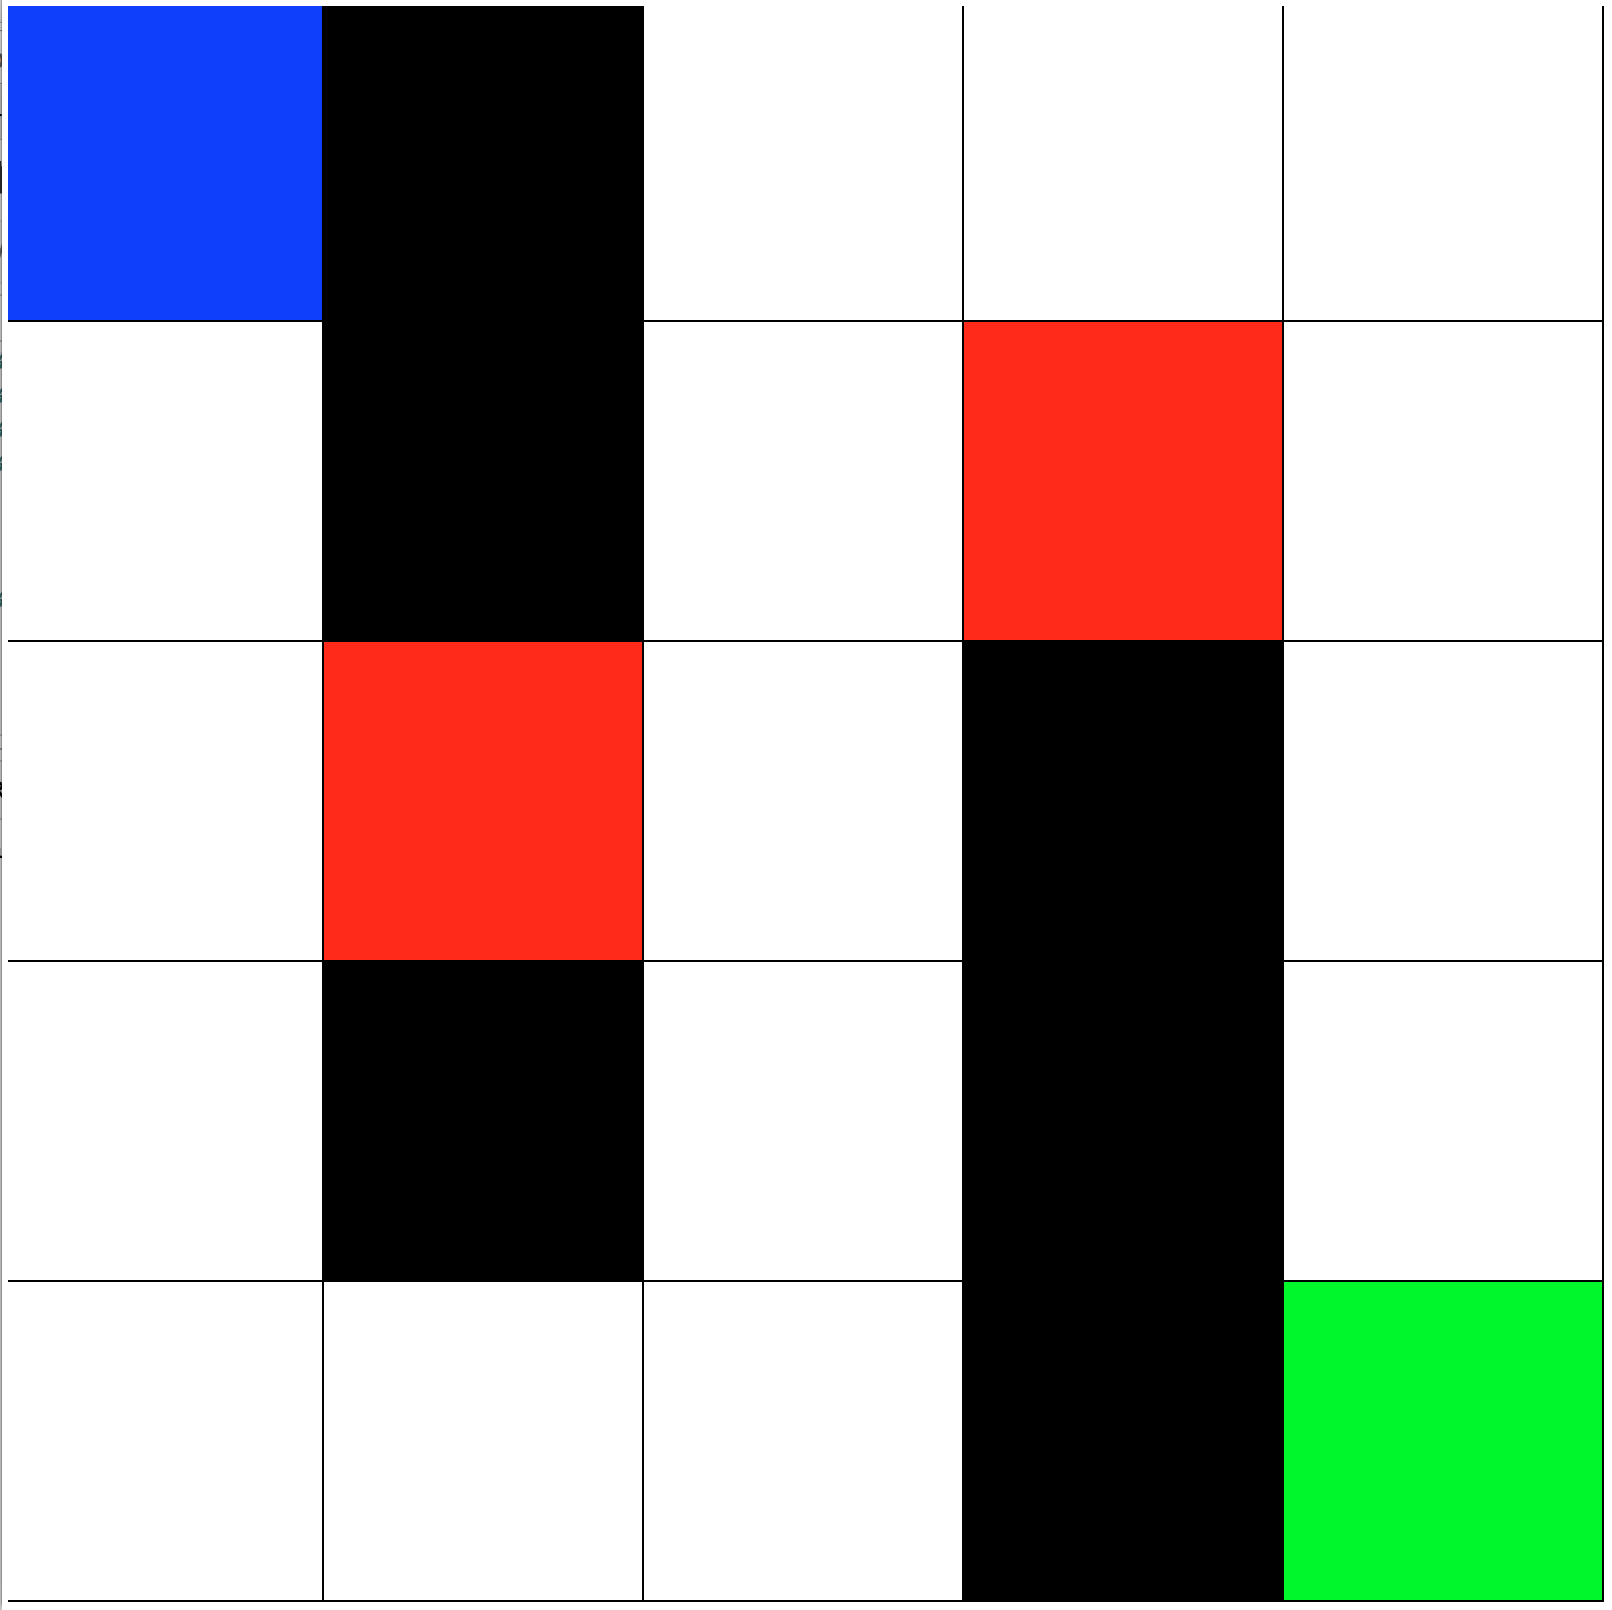
\includegraphics[width=0.5\textwidth]{figures/5by5_nopolicy.png}
\caption{5x5 World}
\end{figure}

The 5x5 gridworld/maze is a small environment used to demonstrate the three techniques. It has a total of 25 possible states that the agent could end up in. Each of the coloured squares in \textit{Figure 1} represents one of the different state types.

\begin{itemize}
\item Blue -- not a state type, indicates the starting position. There are no special rules, rewards, or penalties for entering this state
\item Black -- a wall state
\item Red -- penalty state
\item Green -- goal state
\end{itemize}

\subsubsection{50x50 World}
\begin{figure}[h!]
\centering
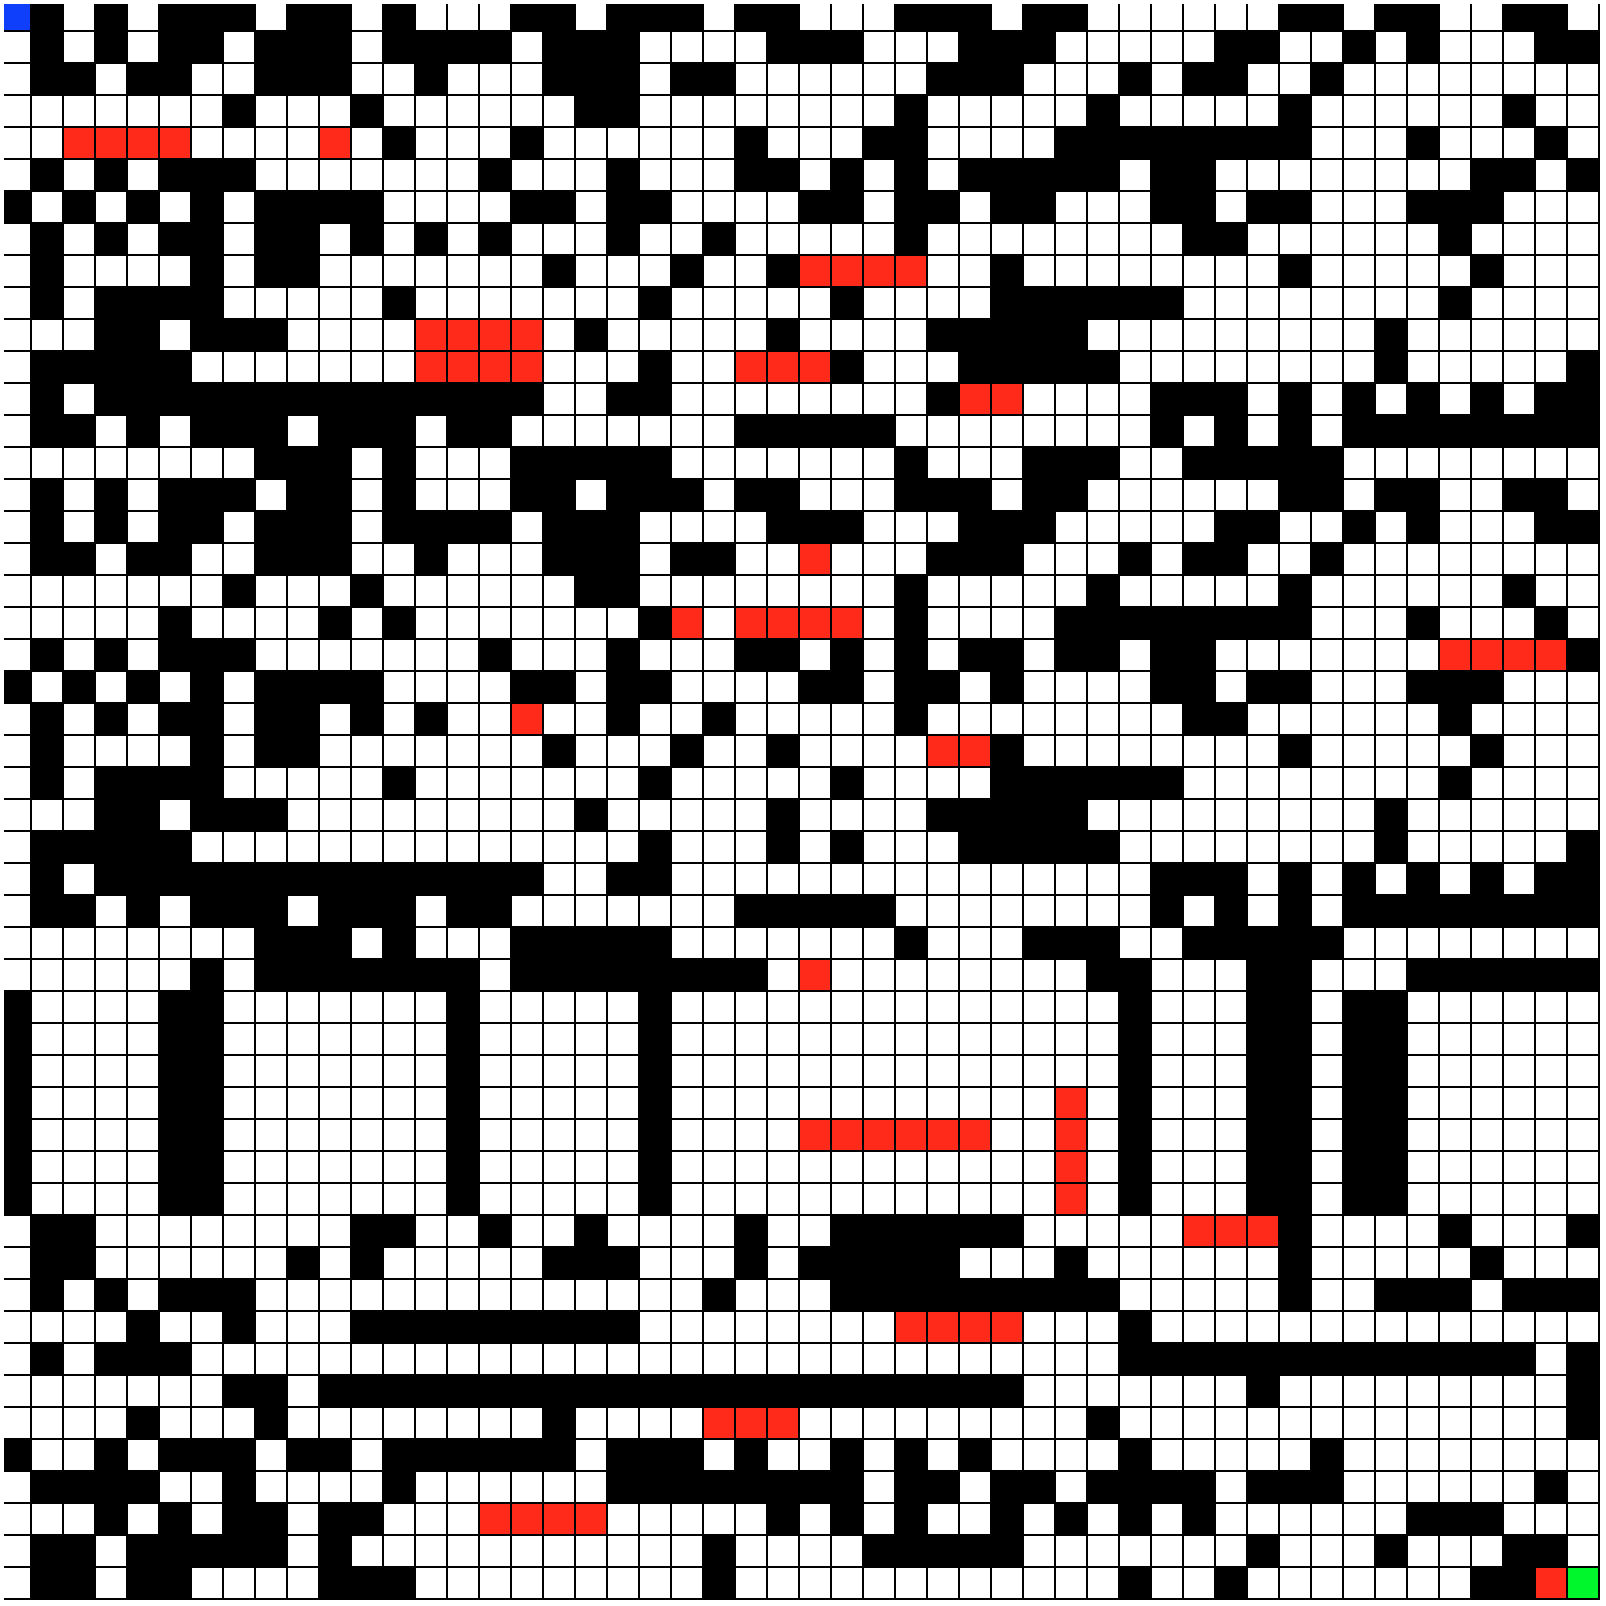
\includegraphics[width=0.5\textwidth]{figures/50by50_nopolicy.png}
\caption{50x50 World}
\end{figure}

The 50x50 gridworld/maze is a larger environment used to demonstrate the three techniques. There are a total of 2500 possible state the agent could end up in. \textit{Figure 2} shows the pseudorandomly generated environment that was generated for experimentation.

\section{Comparisons}
\subsection{5x5 World}
For comparison it is interesting to try each of these methods on different reward schemas. That is, different reward values for: step penalties, entering penalty states, entering the goal states. The reward schema used for applying the three techniques to the 5x5 World will be

\begin{enumerate}
\item Goal State: +10; Step Penalty: -0.05; Penalty State: -1;
\item Goal State: +10; Step Penalty: -1: Penalty State: -5;
\item Goal State: 0; Step Penalty: 1; Penalty State: -2;
\end{enumerate}

\subsubsection{Value Iteration}
\begin{figure}[h!]
        \centering
        \begin{subfigure}[b]{0.3\textwidth}
                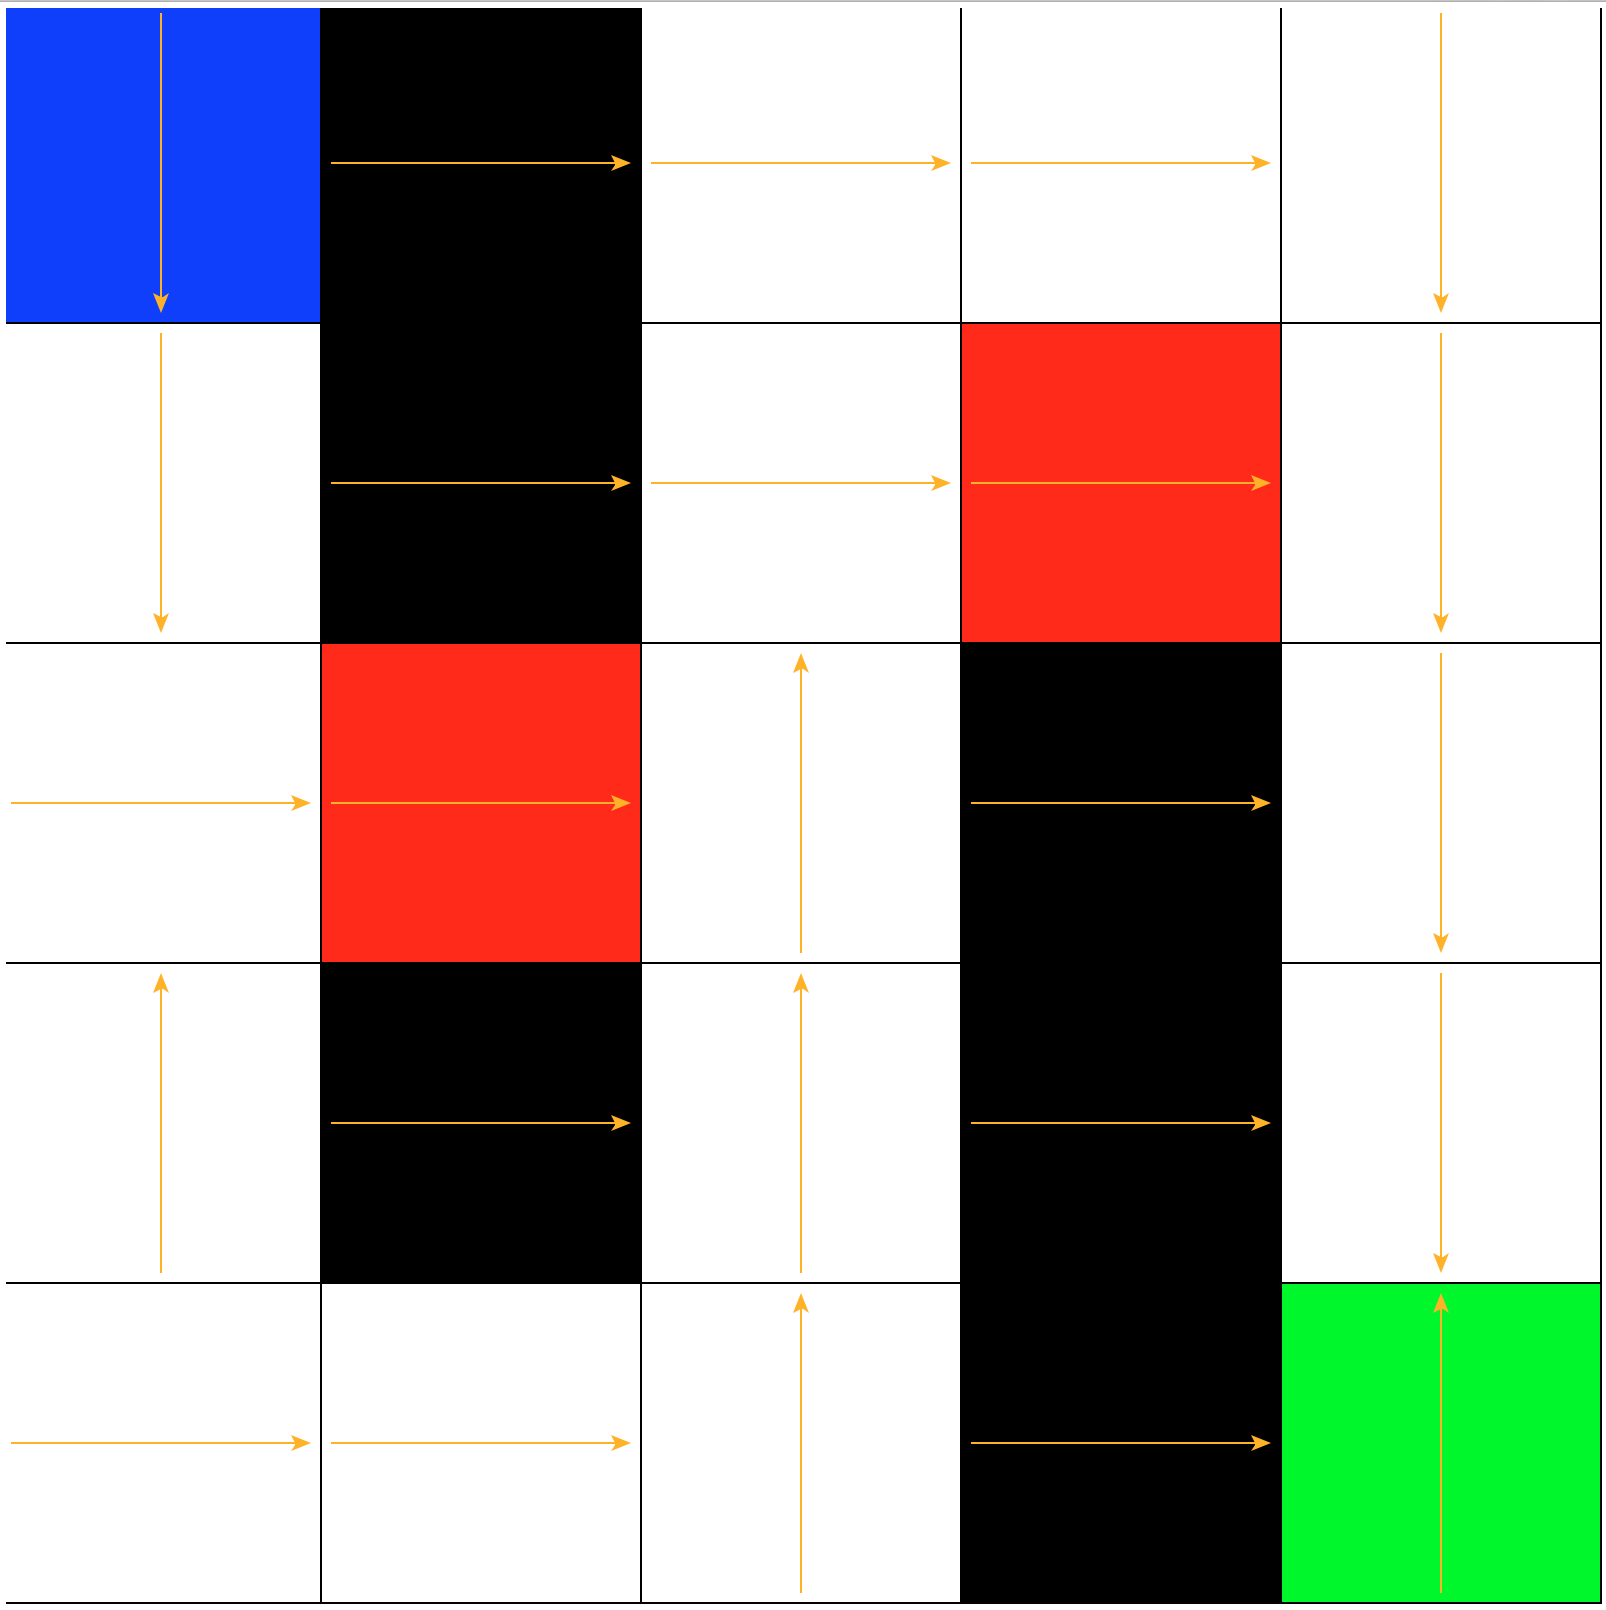
\includegraphics[width=\textwidth]{figures/5x5_viter_r1.png}
                \caption{Reward schema 1\\
                Reward:  7.65\\
                Time:  0.0054\\
                Iterations: 84}
                \label{fig:gull}
        \end{subfigure}%
        ~ %add desired spacing between images, e. g. ~, \quad, \qquad, \hfill etc.
          %(or a blank line to force the subfigure onto a new line)
        \begin{subfigure}[b]{0.3\textwidth}
                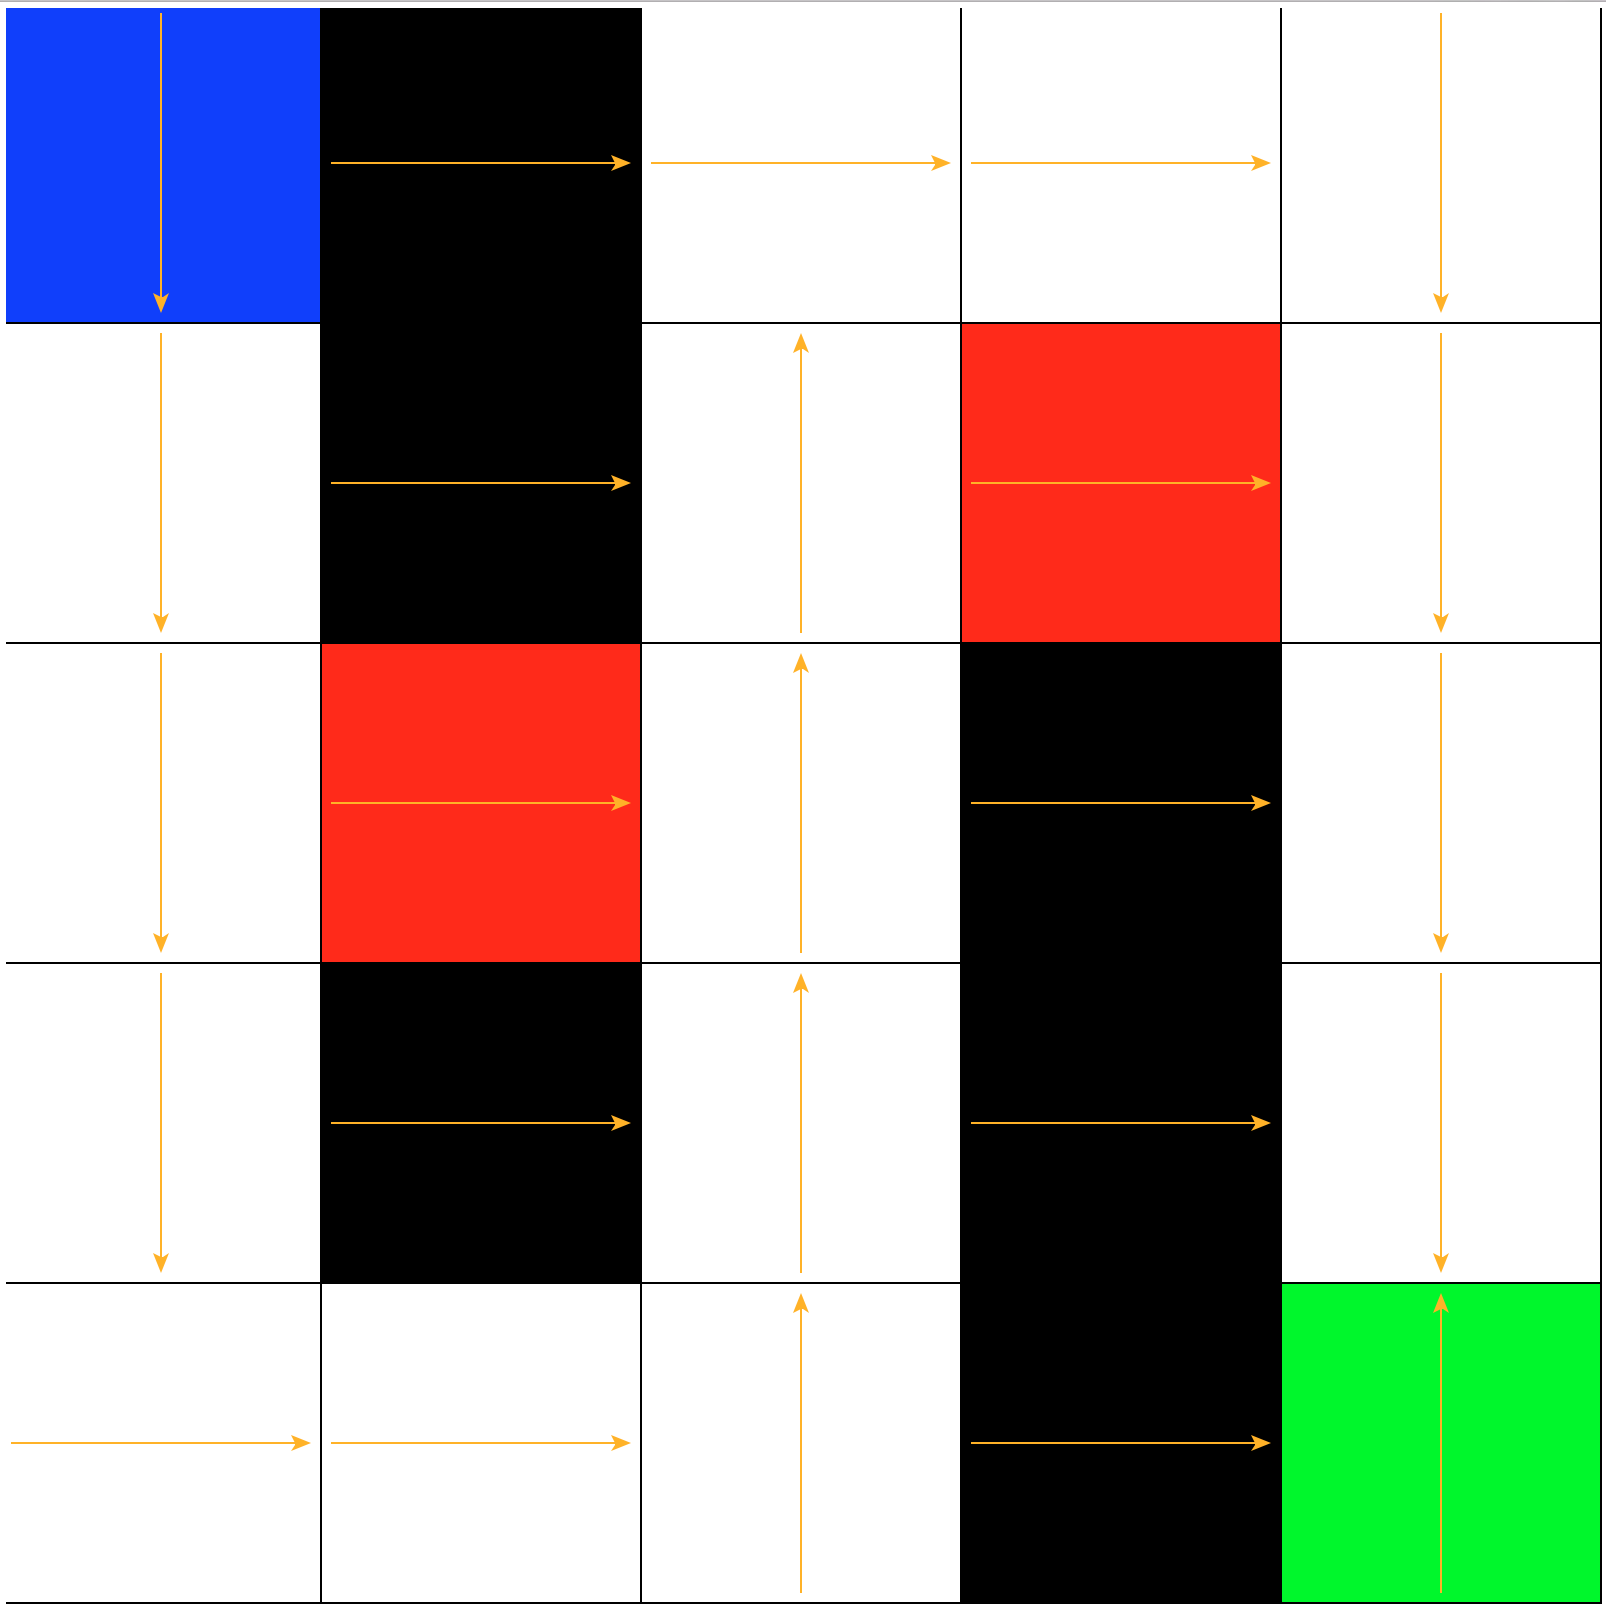
\includegraphics[width=\textwidth]{figures/5x5_viter_r2.png}
                \caption{Reward schema 2\\
                Reward: -5 \\
                Time:  0.0061\\
                Iterations: 81}
                \label{fig:tiger}
        \end{subfigure}
        ~ %add desired spacing between images, e. g. ~, \quad, \qquad, \hfill etc.
          %(or a blank line to force the subfigure onto a new line)
        \begin{subfigure}[b]{0.3\textwidth}
                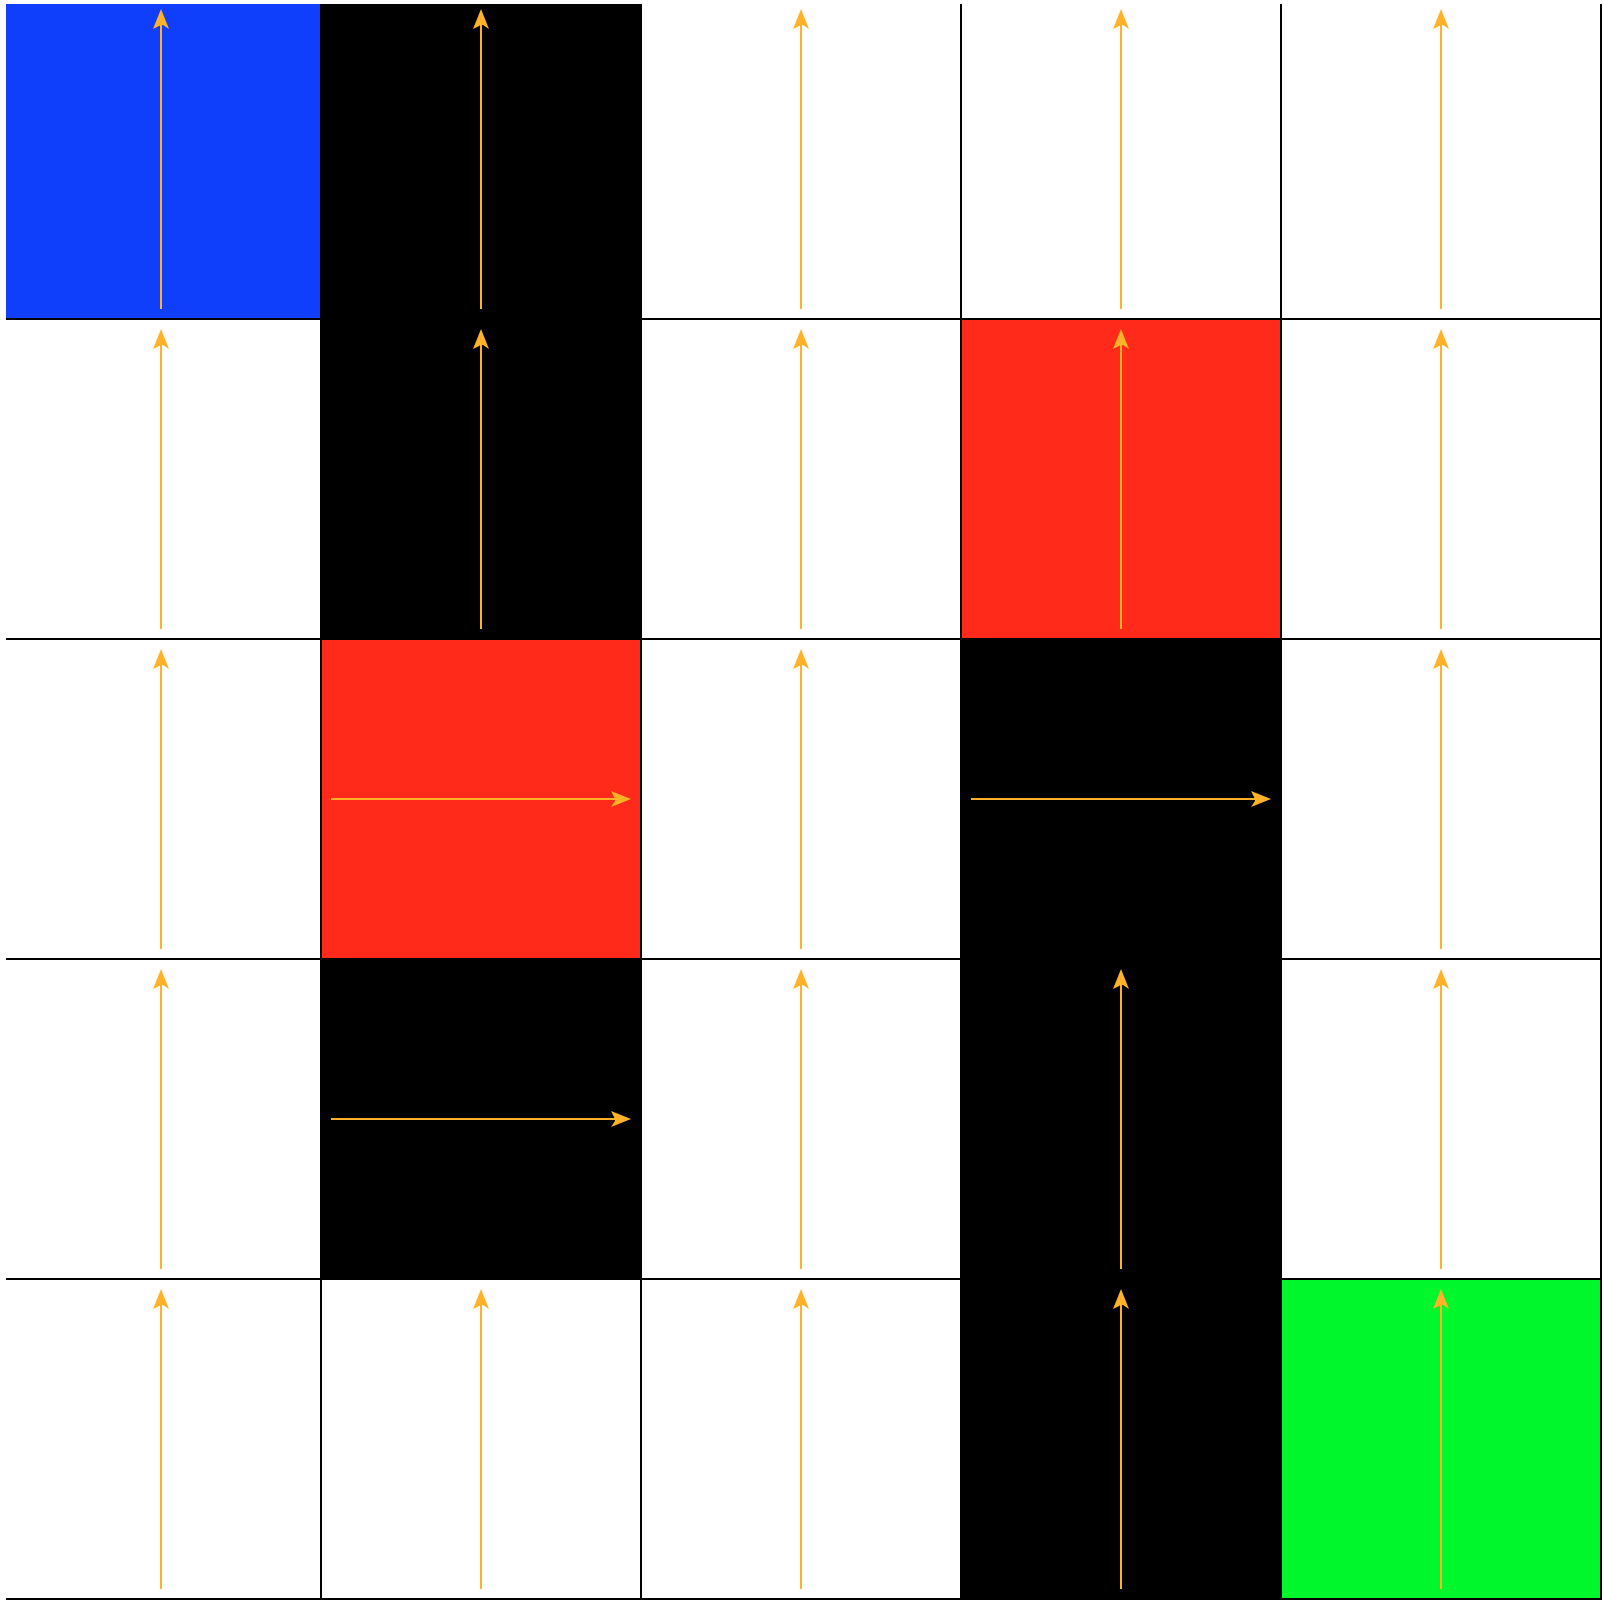
\includegraphics[width=\textwidth]{figures/5x5_viter_r3.png}
                \caption{Reward schema 3\\
                Reward: $\infty$  \\
                Time:  0.0002\\
                Iterations: 2}
                \label{fig:mouse}
        \end{subfigure}
        \caption{Policies Learned by Value Iteration}\label{fig:animals}
\end{figure}

\subsubsection{Policy Iteration}
\begin{figure}[h!]
        \centering
        \begin{subfigure}[b]{0.3\textwidth}
                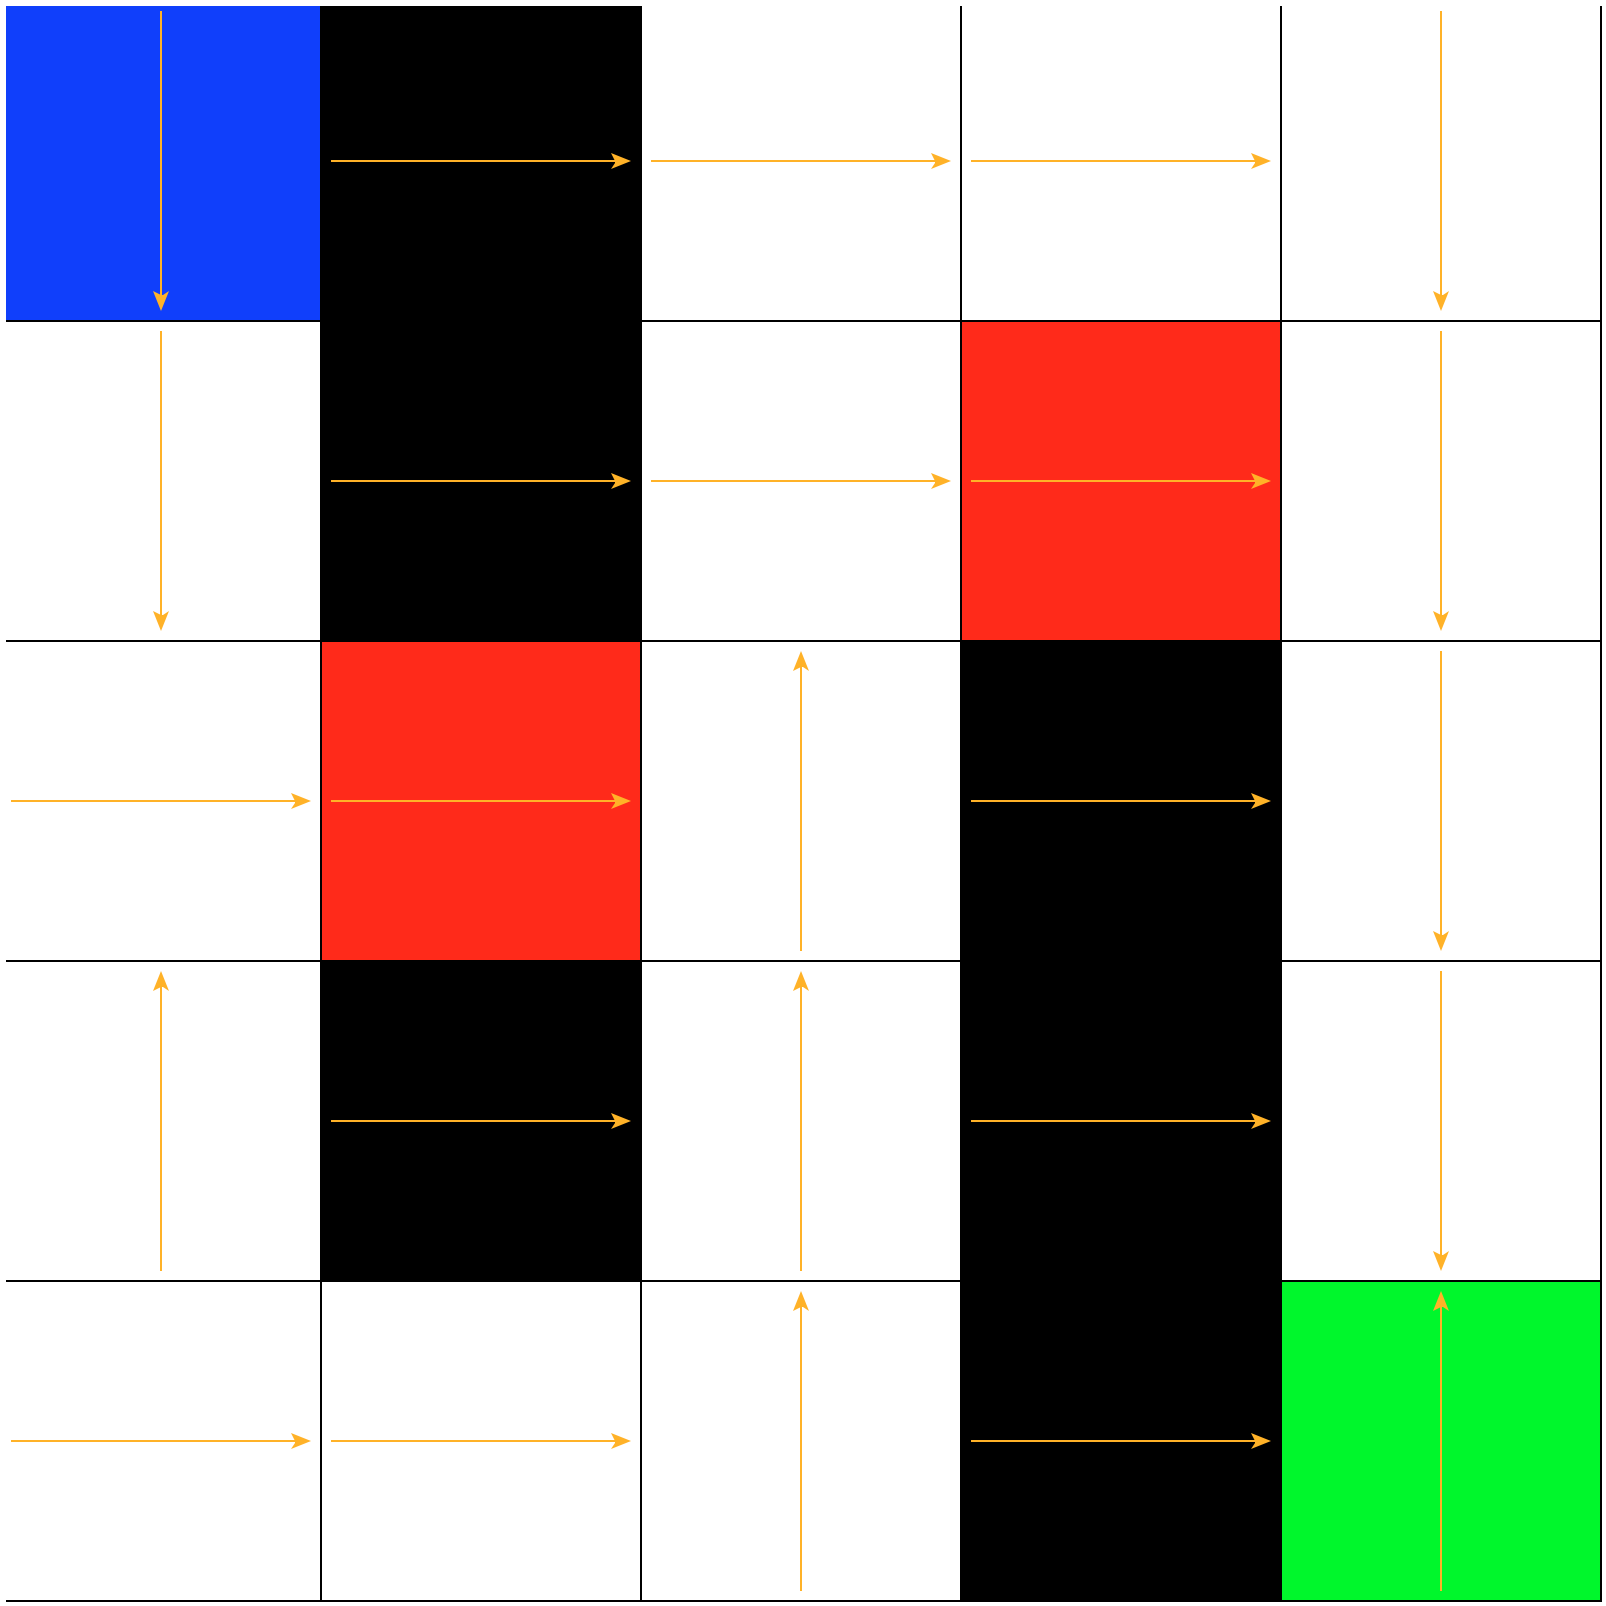
\includegraphics[width=\textwidth]{figures/5x5_piter_r1.png}
                \caption{Reward schema 1\\
                Reward:  7.65 \\
                Time:  0.0094\\
                Iterations: 10 }
                \label{fig:gull}
        \end{subfigure}%
        ~ %add desired spacing between images, e. g. ~, \quad, \qquad, \hfill etc.
          %(or a blank line to force the subfigure onto a new line)
        \begin{subfigure}[b]{0.3\textwidth}
                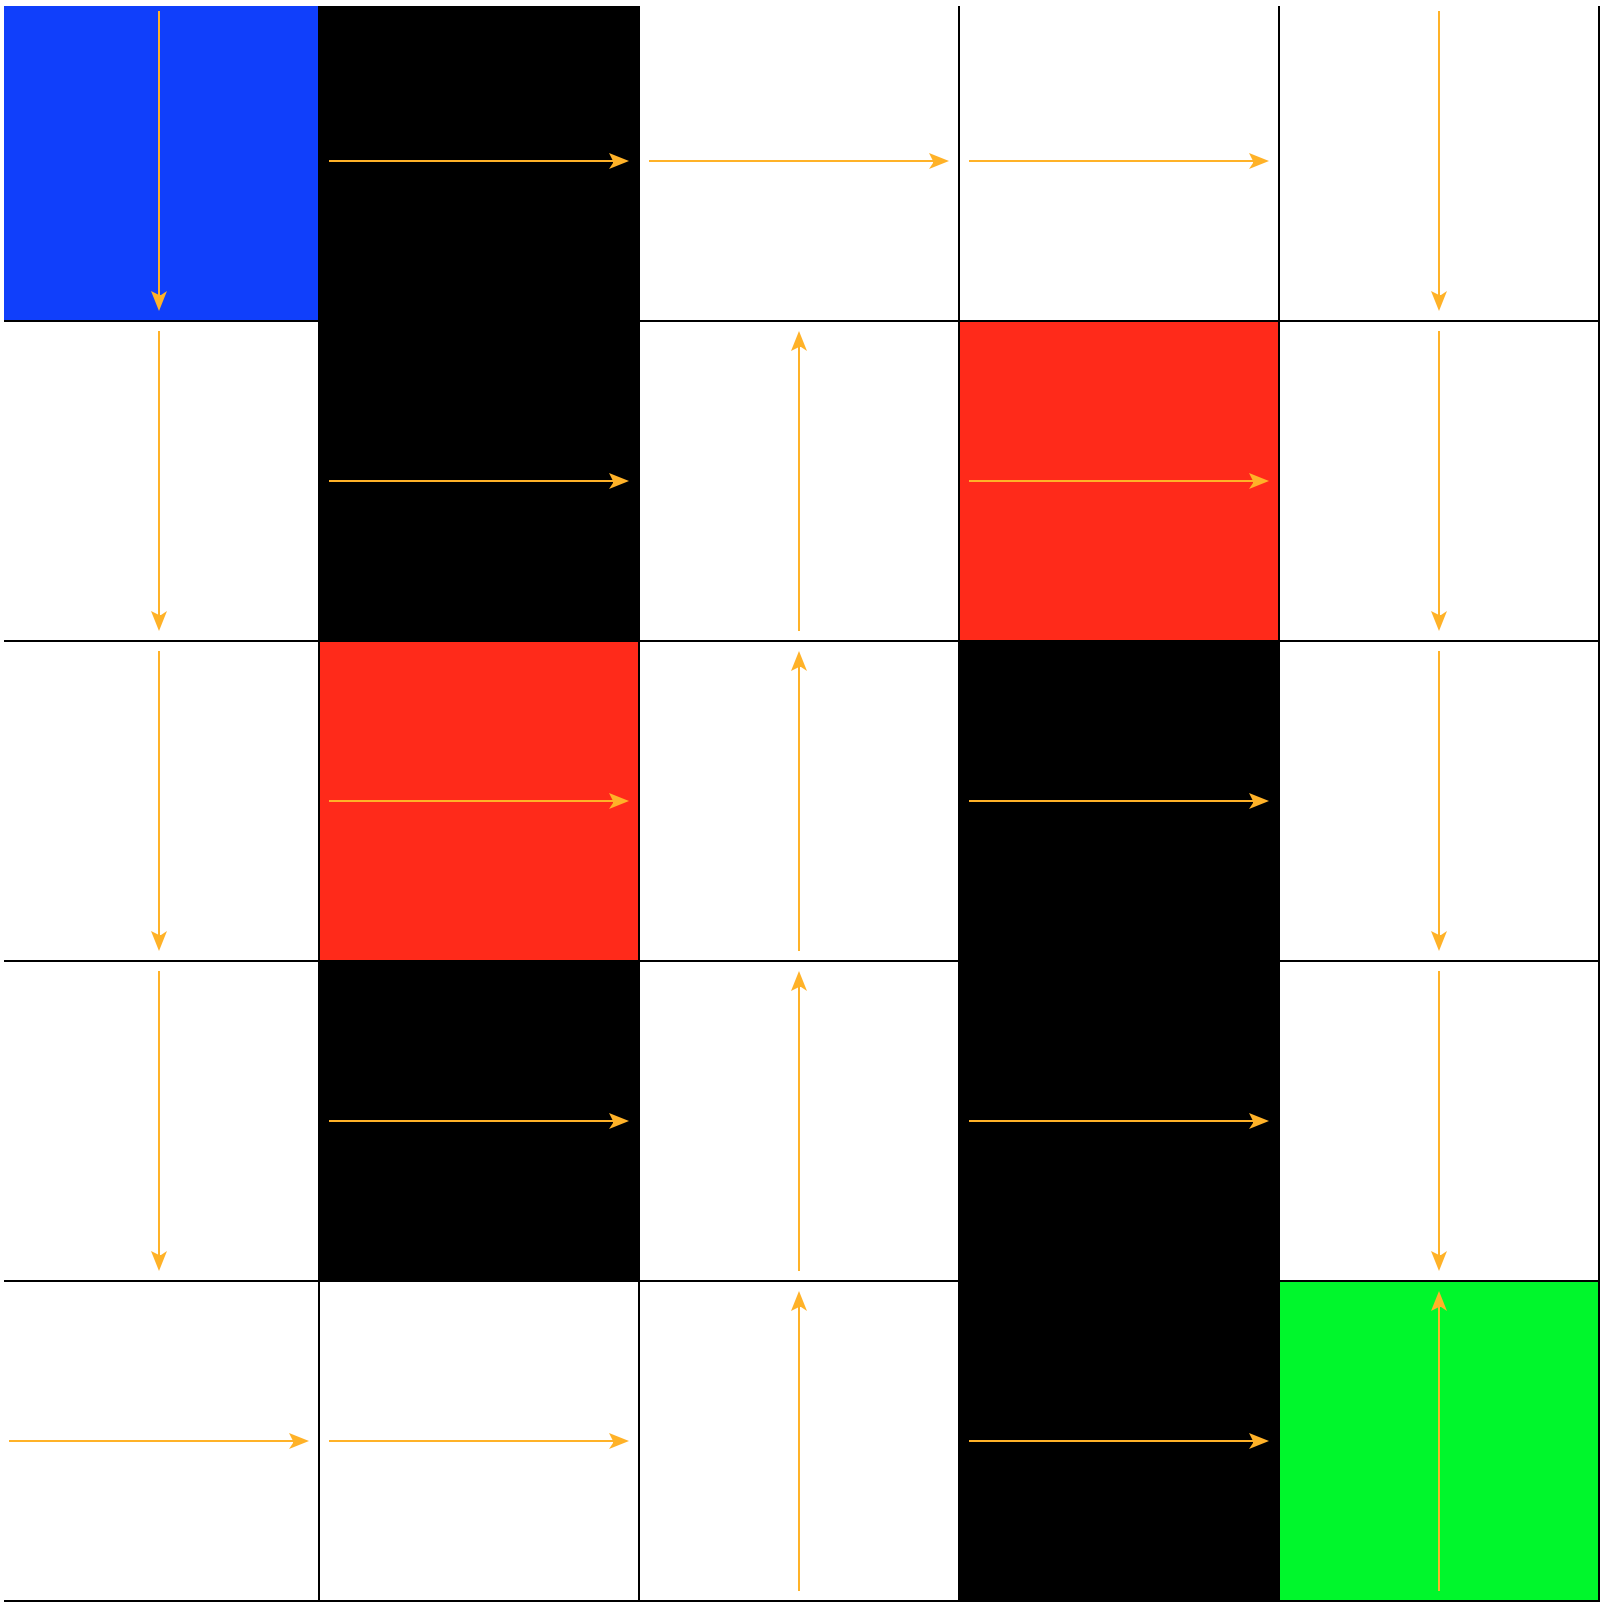
\includegraphics[width=\textwidth]{figures/5x5_piter_r2.png}
                \caption{Reward schema 2\\
                Reward: -5 \\
                Time:  0.0112\\
                Iterations: 11 }
                \label{fig:tiger}
        \end{subfigure}
        ~ %add desired spacing between images, e. g. ~, \quad, \qquad, \hfill etc.
          %(or a blank line to force the subfigure onto a new line)
        \begin{subfigure}[b]{0.3\textwidth}
                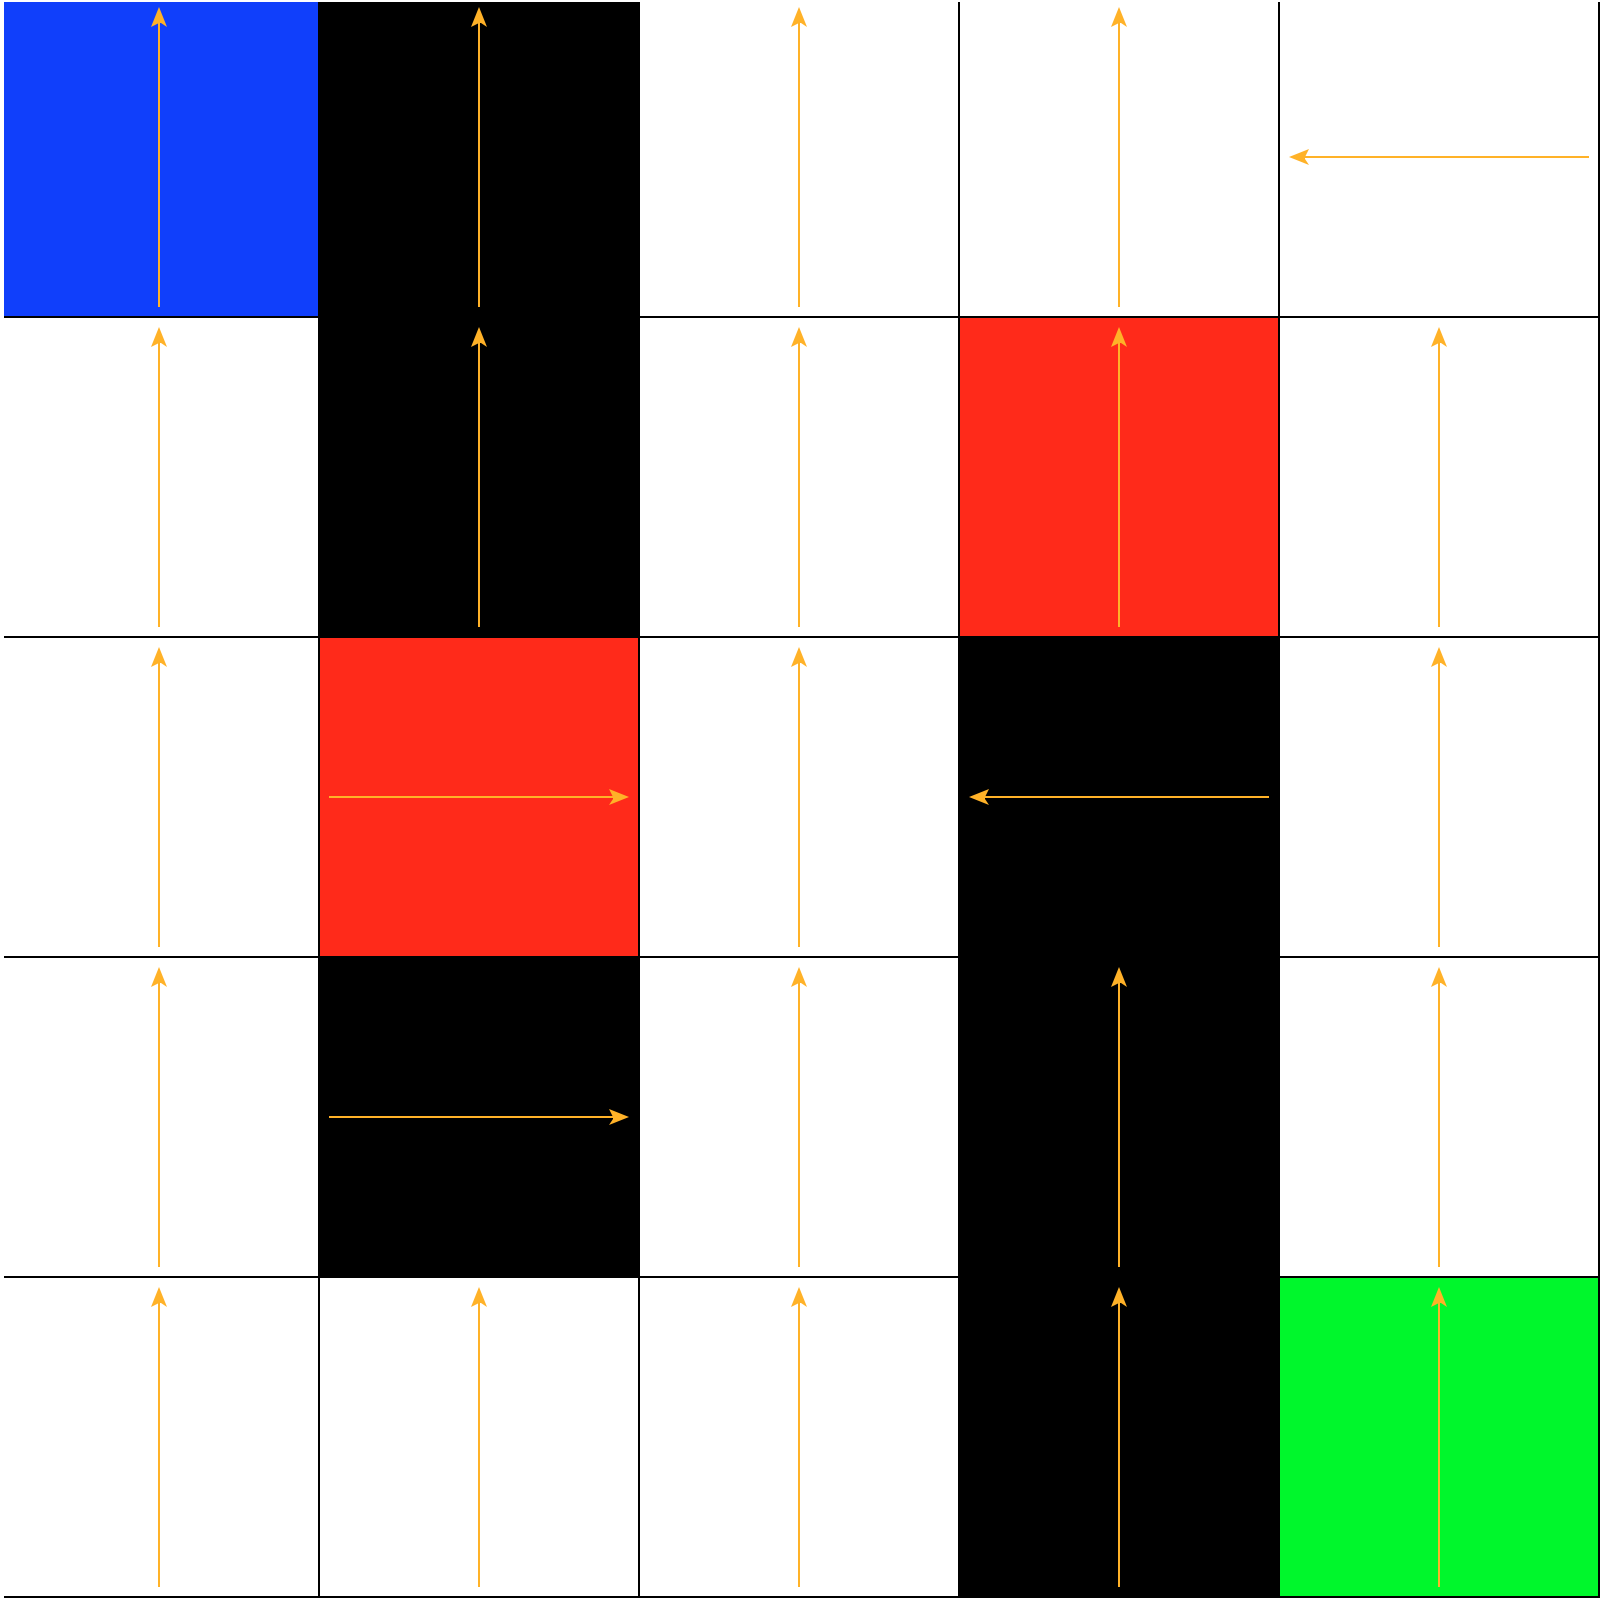
\includegraphics[width=\textwidth]{figures/5x5_piter_r3.png}
                \caption{Reward schema 3\\
                Reward: $\infty$ \\
                Time: 0.5076\\
                Iterations: 1000 (max)}
                \label{fig:mouse}
        \end{subfigure}
        \caption{Policies Learned by Policy Iteration}\label{fig:animals}
\end{figure}

\subsubsection{Q-Learning}
\begin{figure}[h!]
        \centering
        \begin{subfigure}[b]{0.3\textwidth}
                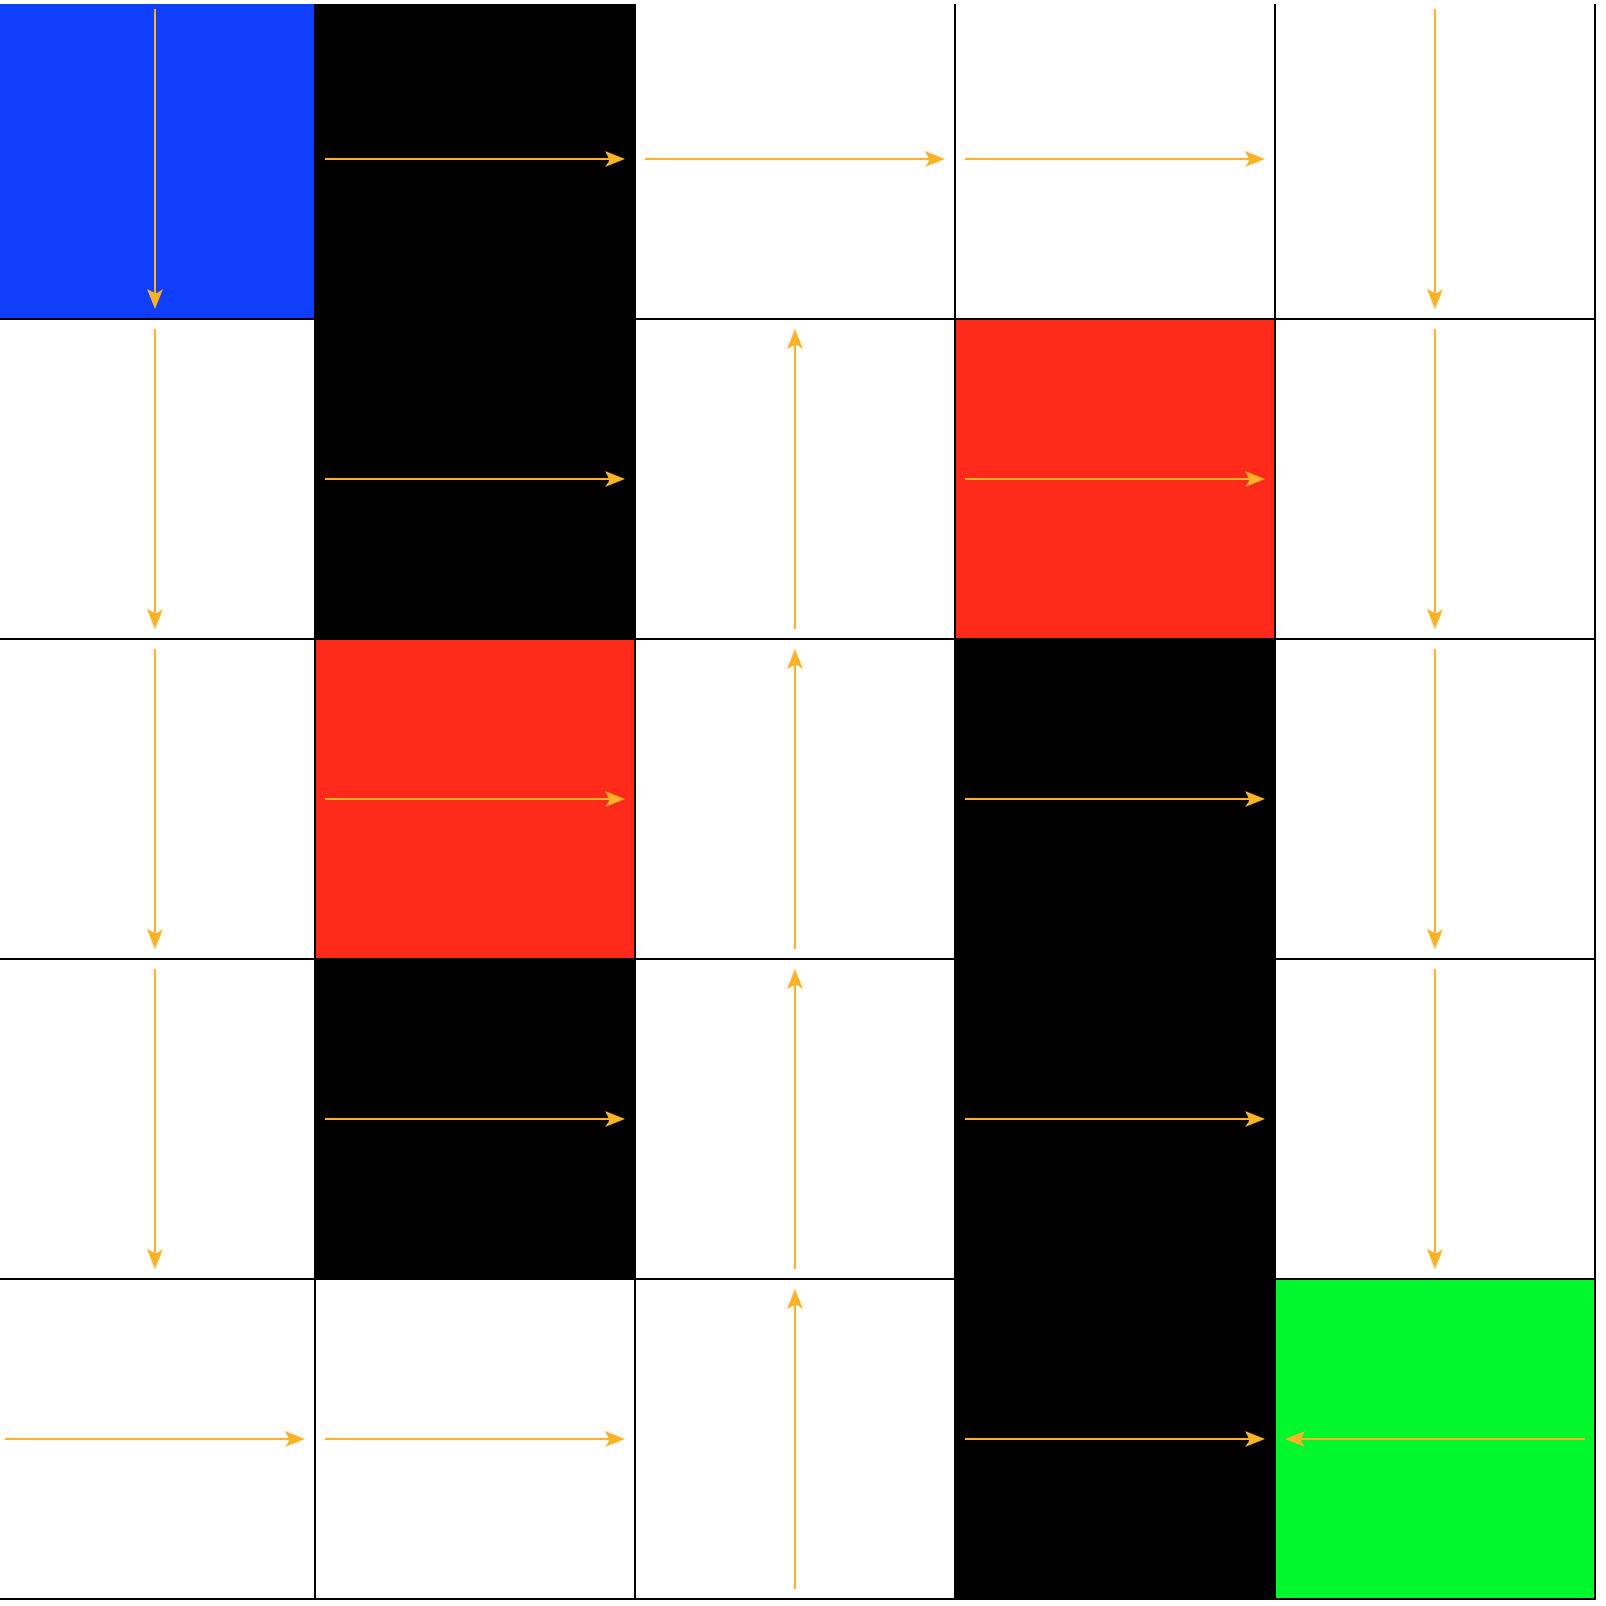
\includegraphics[width=\textwidth]{figures/5x5_qlearn_r1.png}
                \caption{Reward schema 1\\ 
                Reward:  9.25 \\
                Time:  1.353 \\
                Iterations:  25013 }
                \label{fig:gull}
        \end{subfigure}%
        ~ %add desired spacing between images, e. g. ~, \quad, \qquad, \hfill etc.
          %(or a blank line to force the subfigure onto a new line)
        \begin{subfigure}[b]{0.3\textwidth}
                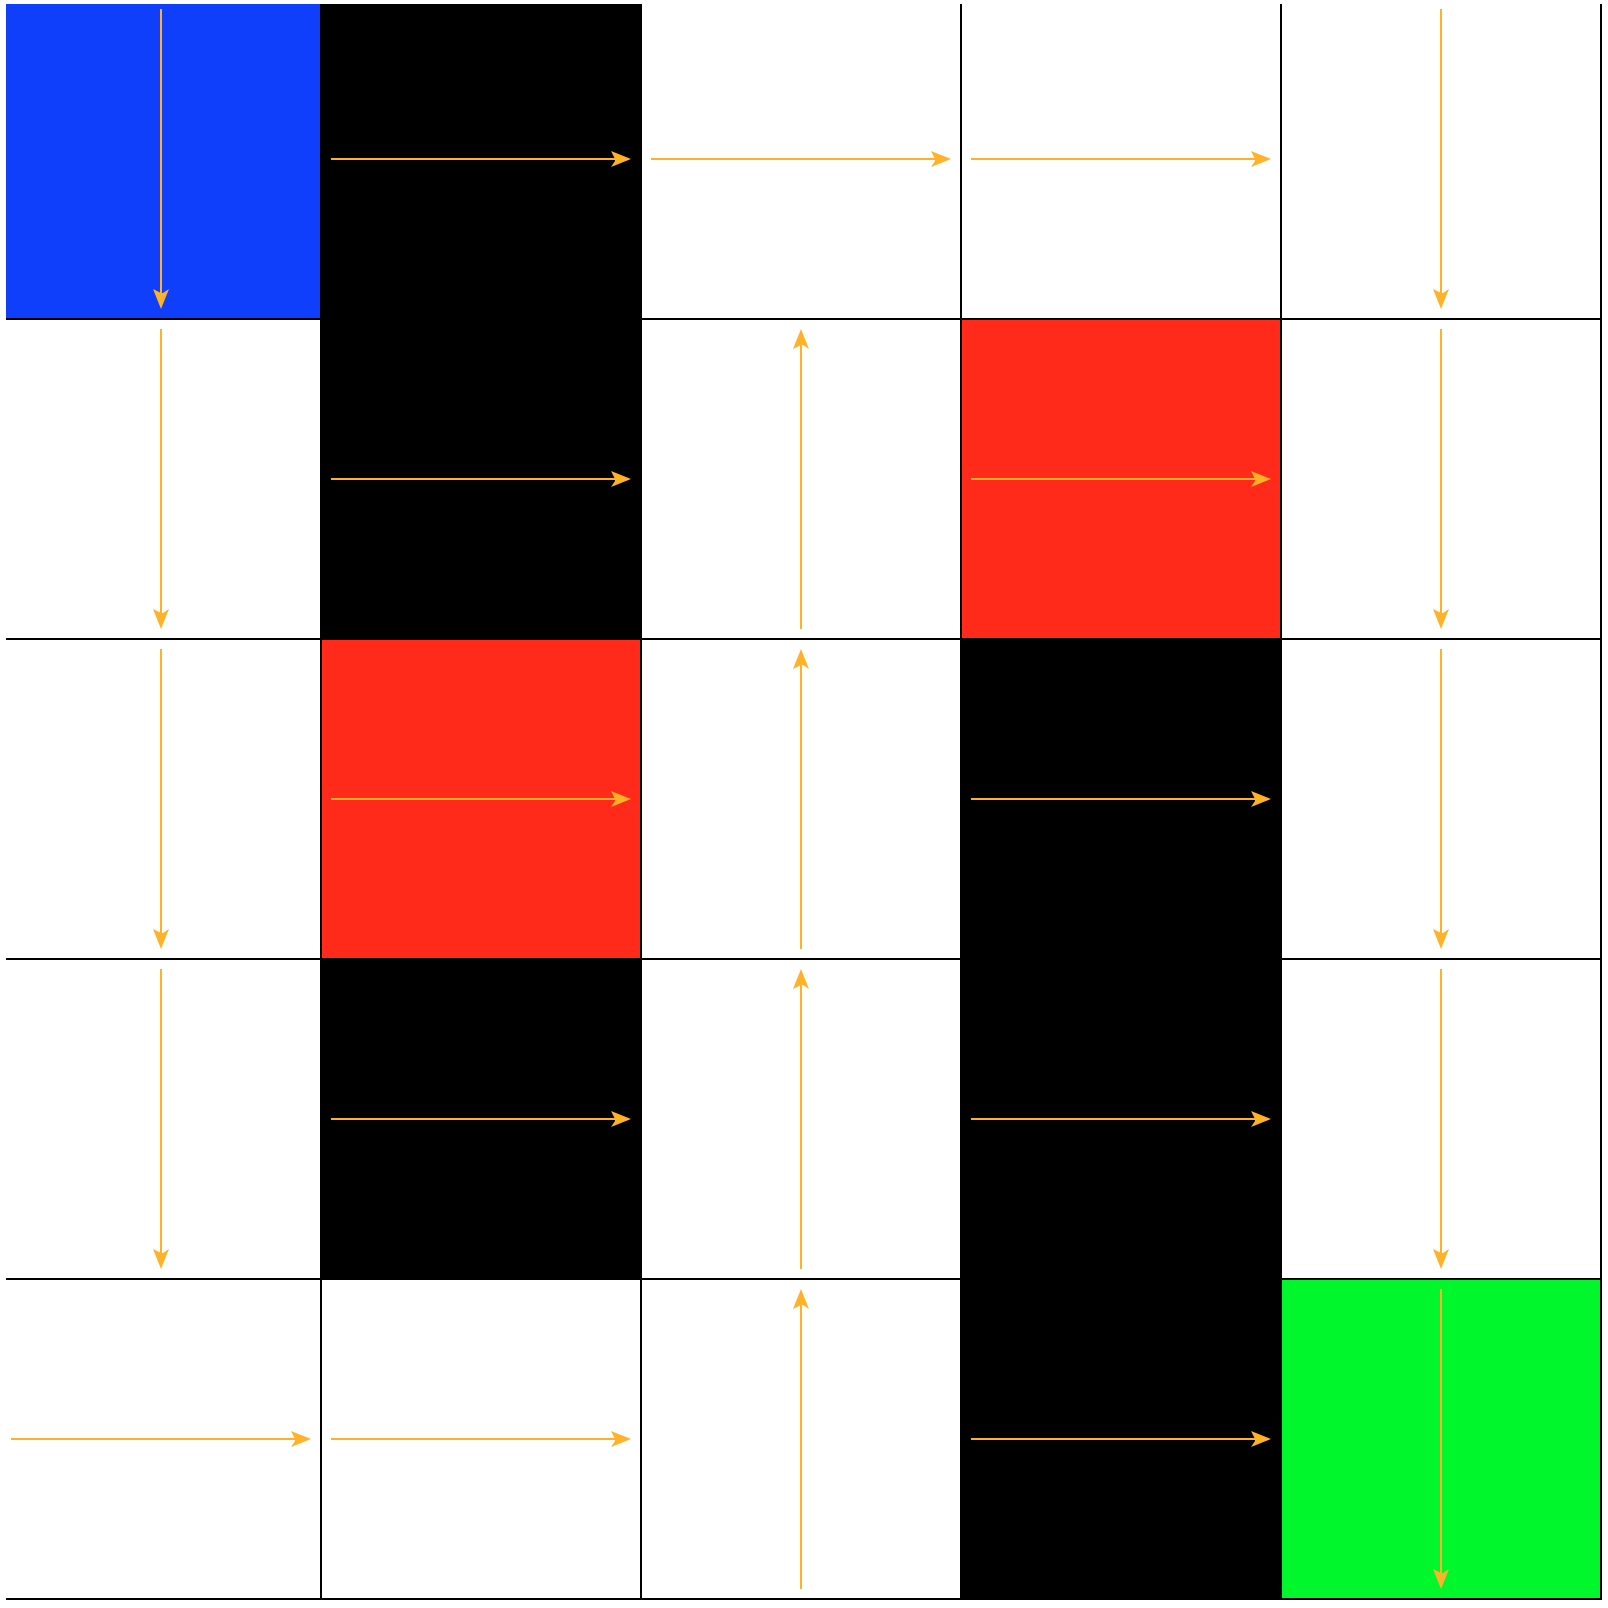
\includegraphics[width=\textwidth]{figures/5x5_qlearn_r2.png}
                \caption{Reward schema 2\\
                Reward: -5\\
                Time:  1.340\\
                Iterations: 25597 }
                \label{fig:tiger}
        \end{subfigure}
        ~ %add desired spacing between images, e. g. ~, \quad, \qquad, \hfill etc.
          %(or a blank line to force the subfigure onto a new line)
        \begin{subfigure}[b]{0.3\textwidth}
                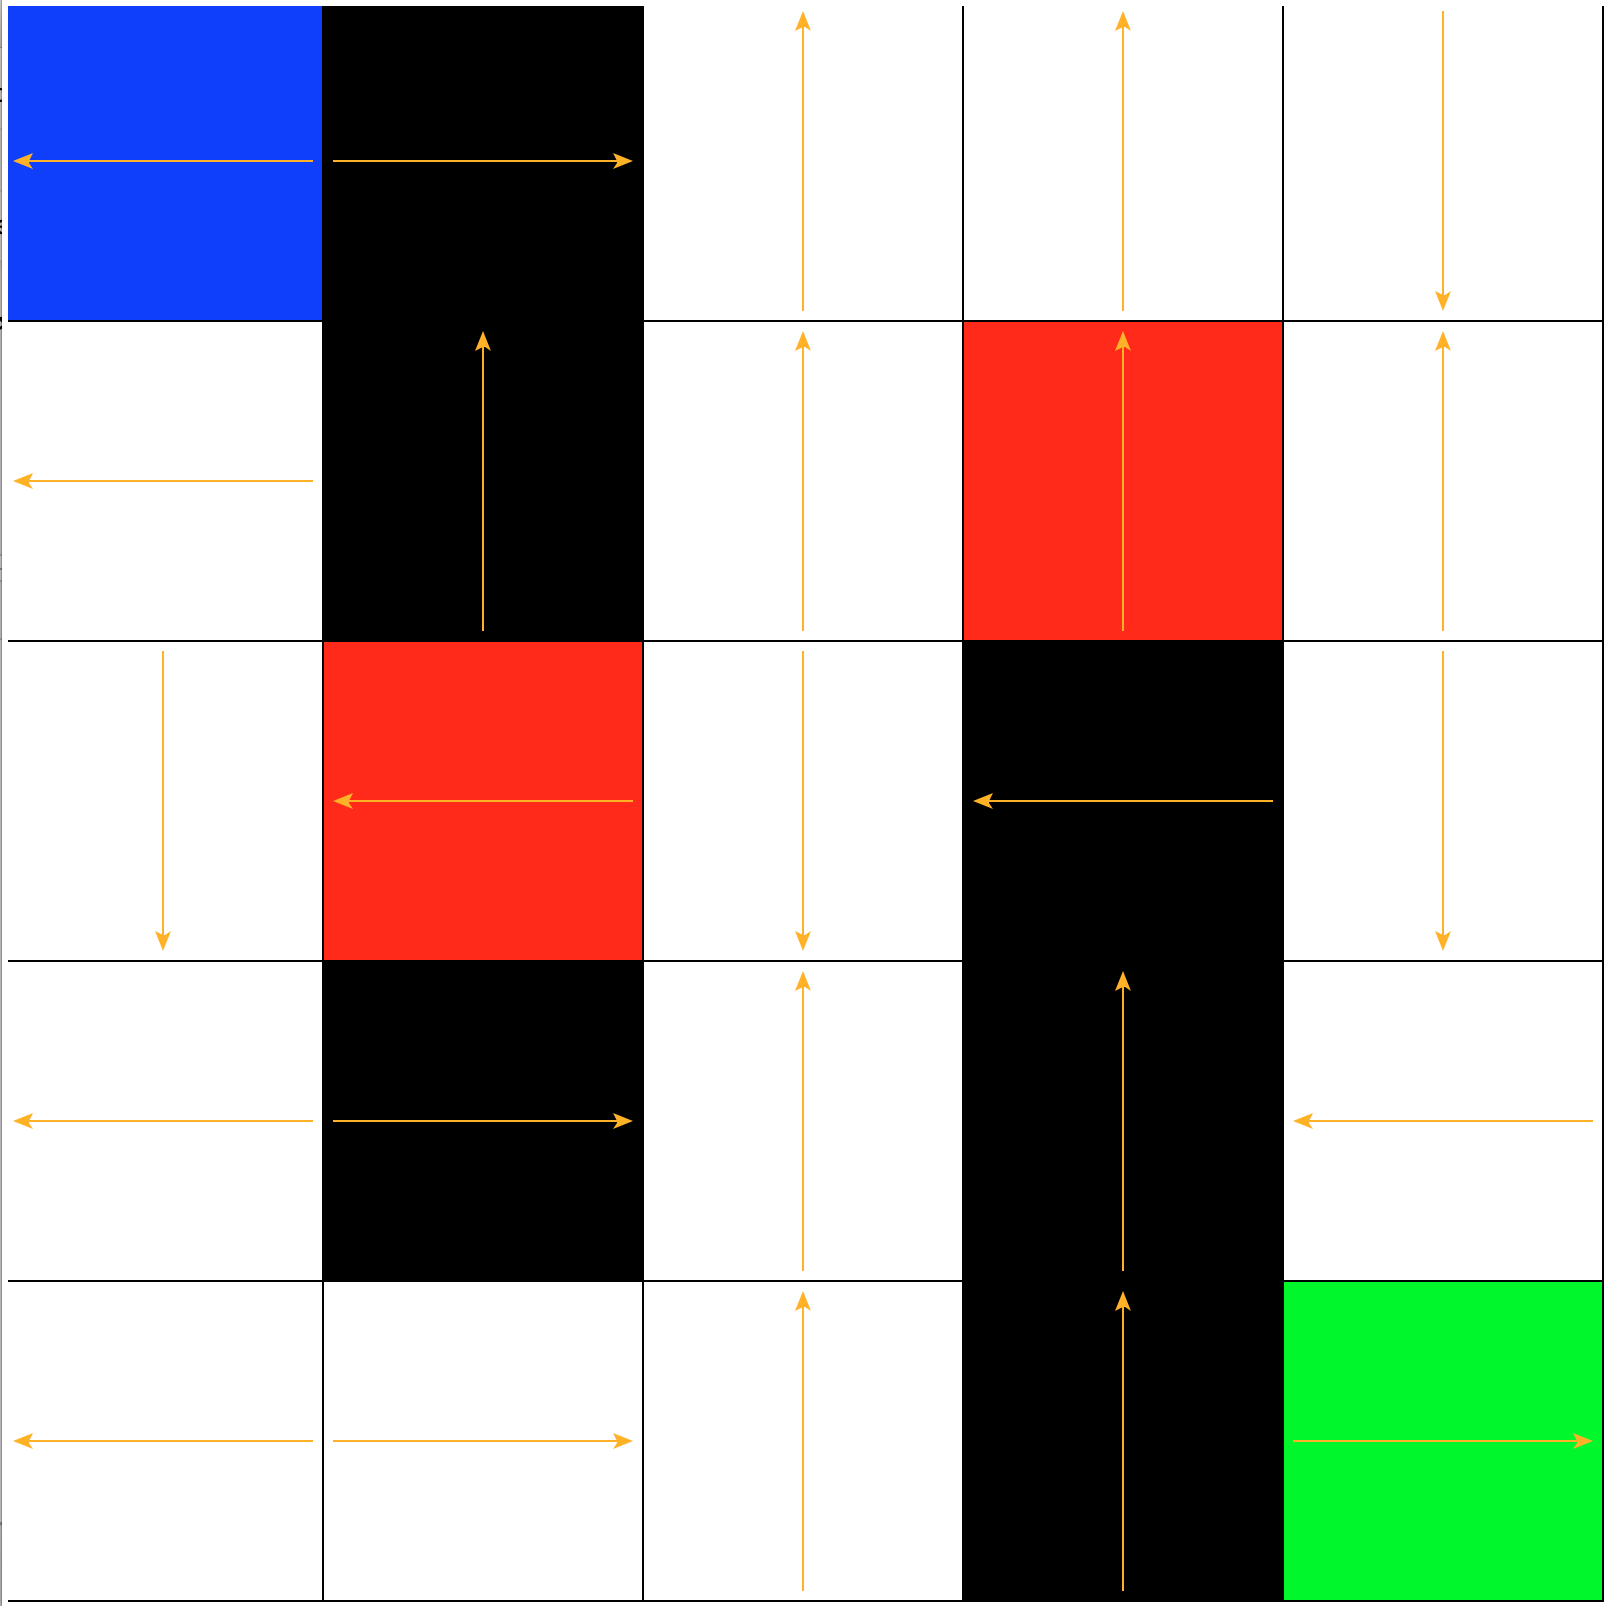
\includegraphics[width=\textwidth]{figures/5x5_qlearn_r3.png}
                \caption{Reward schema 3 \\
                Reward: $\infty$\\
                Time: 1.677 \\
                Iterations: 65465 }
                \label{fig:mouse}
        \end{subfigure}
        \caption{Policies Learned by Q-Learning}\label{fig:animals}
\end{figure}

\subsection{50x50 World}

\subsubsection{Value Iteration}
\begin{figure}[h!]
        \centering
        \begin{subfigure}[b]{0.3\textwidth}
                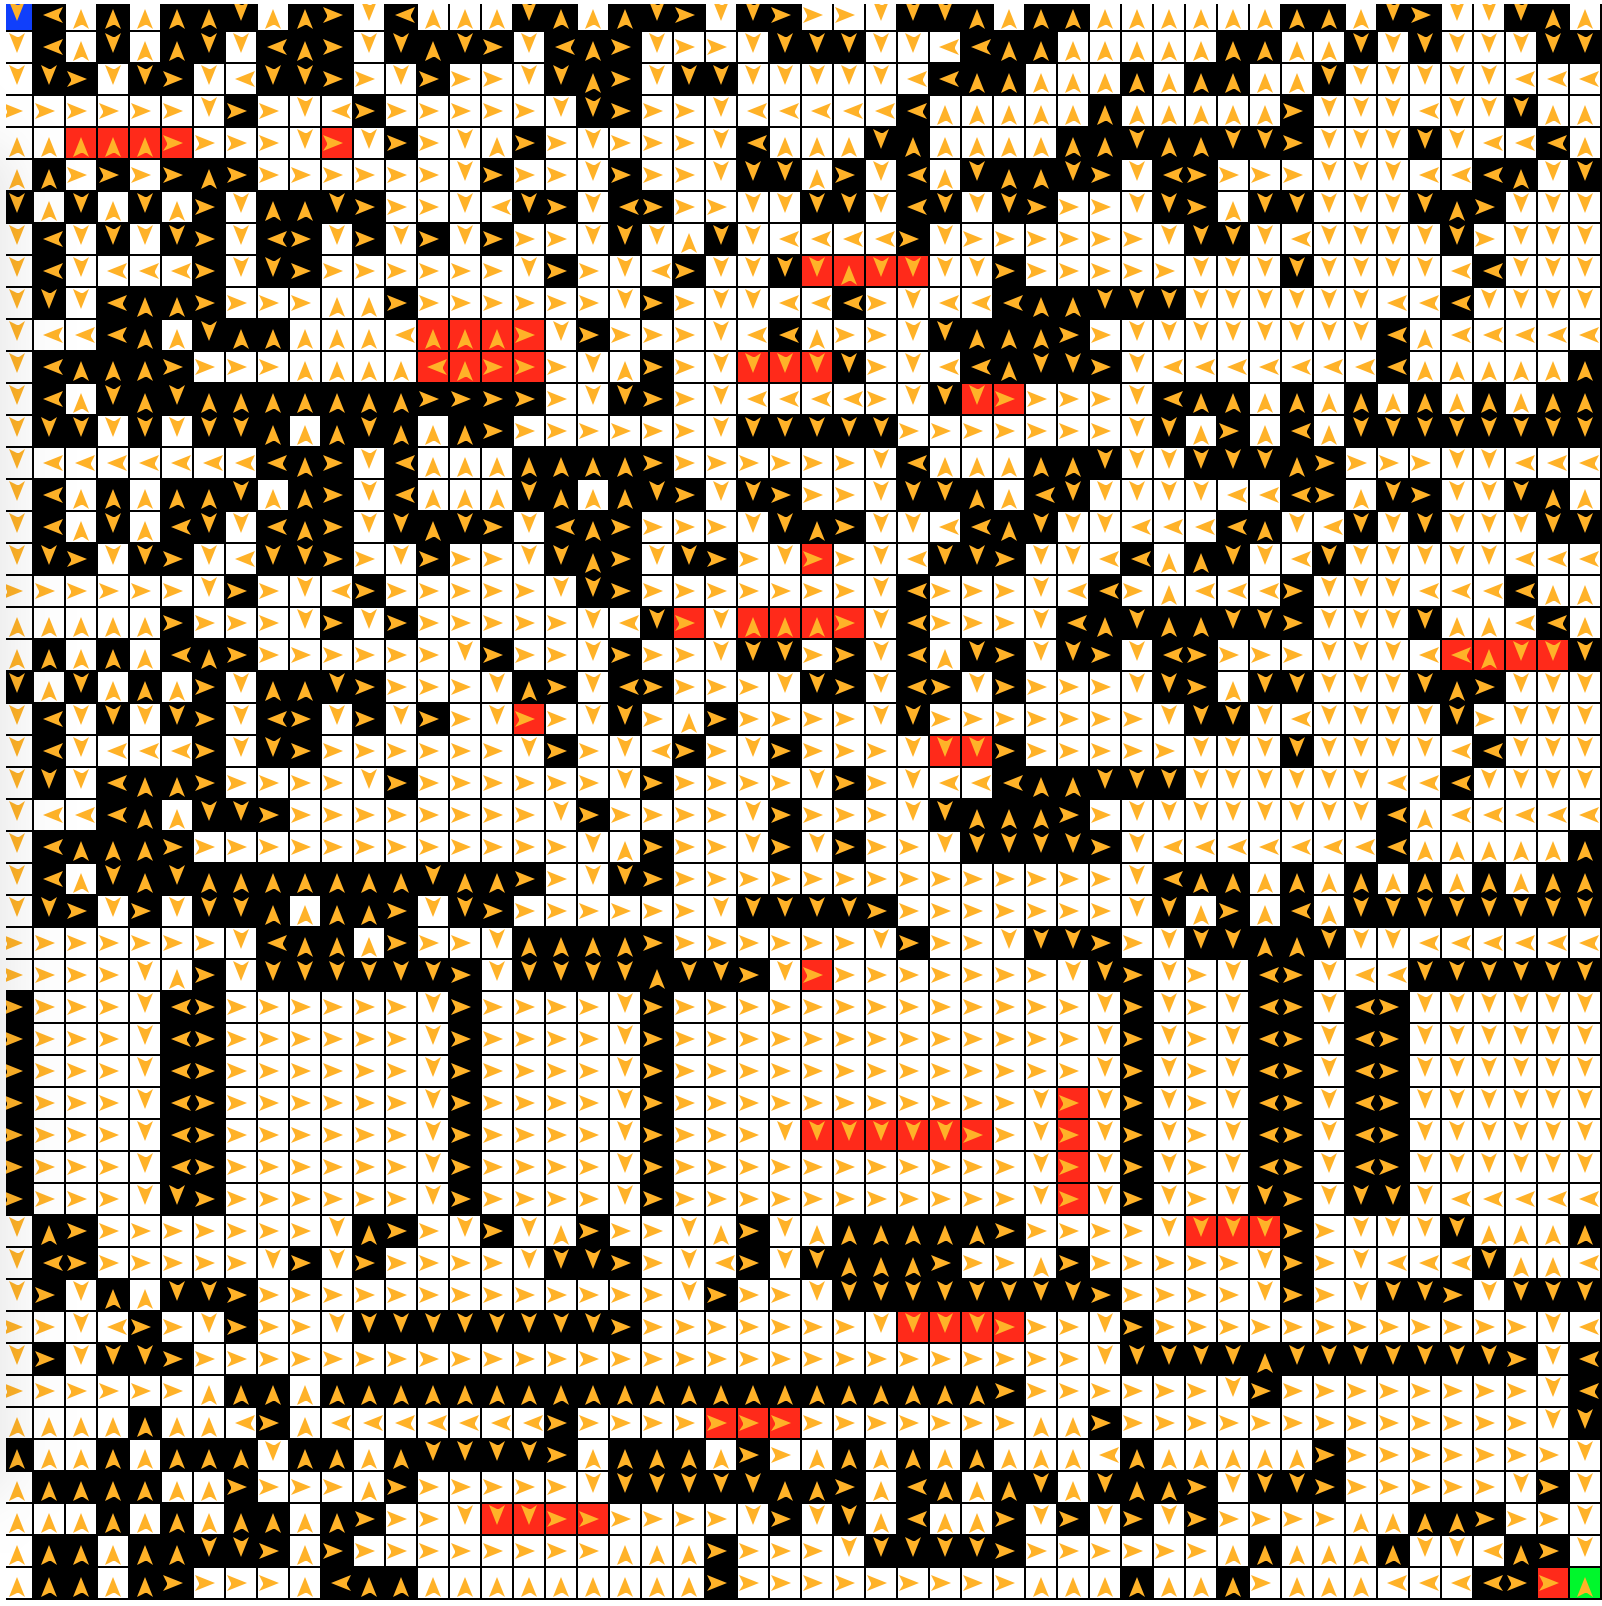
\includegraphics[width=\textwidth]{figures/50x50_viter_r1.png}
                \caption{Reward schema 1\\
                Reward:  995.15\\
                Time:  1.5505\\
                Iterations: 131}
                \label{fig:gull}
        \end{subfigure}%
        ~ %add desired spacing between images, e. g. ~, \quad, \qquad, \hfill etc.
          %(or a blank line to force the subfigure onto a new line)
        \begin{subfigure}[b]{0.3\textwidth}
                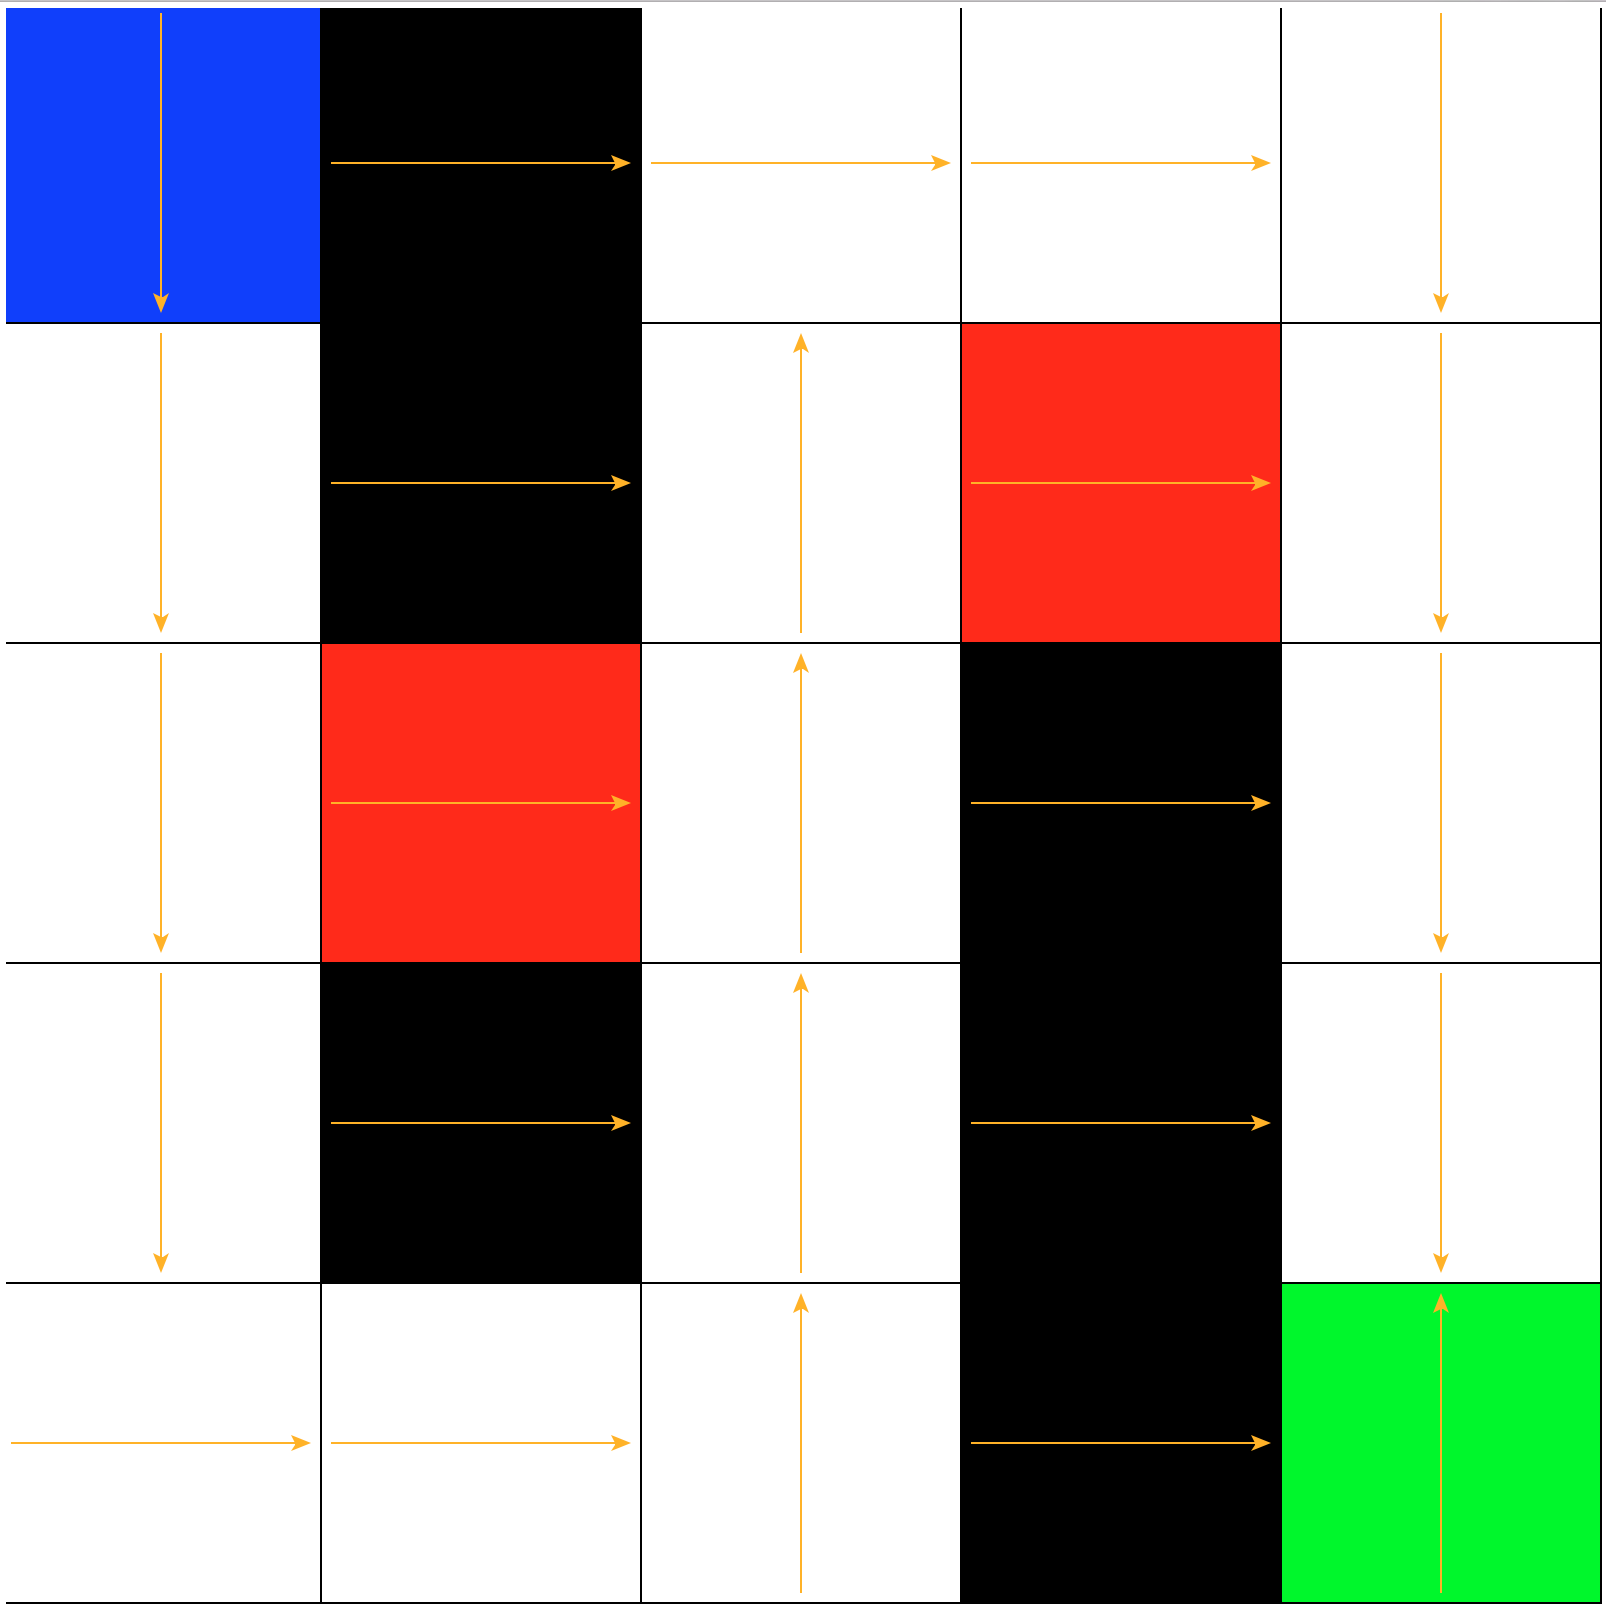
\includegraphics[width=\textwidth]{figures/5x5_viter_r2.png}
                \caption{Reward schema 2\\
                Reward: -5 \\
                Time:  0.0061\\
                Iterations: 81}
                \label{fig:tiger}
        \end{subfigure}
        ~ %add desired spacing between images, e. g. ~, \quad, \qquad, \hfill etc.
          %(or a blank line to force the subfigure onto a new line)
        \begin{subfigure}[b]{0.3\textwidth}
                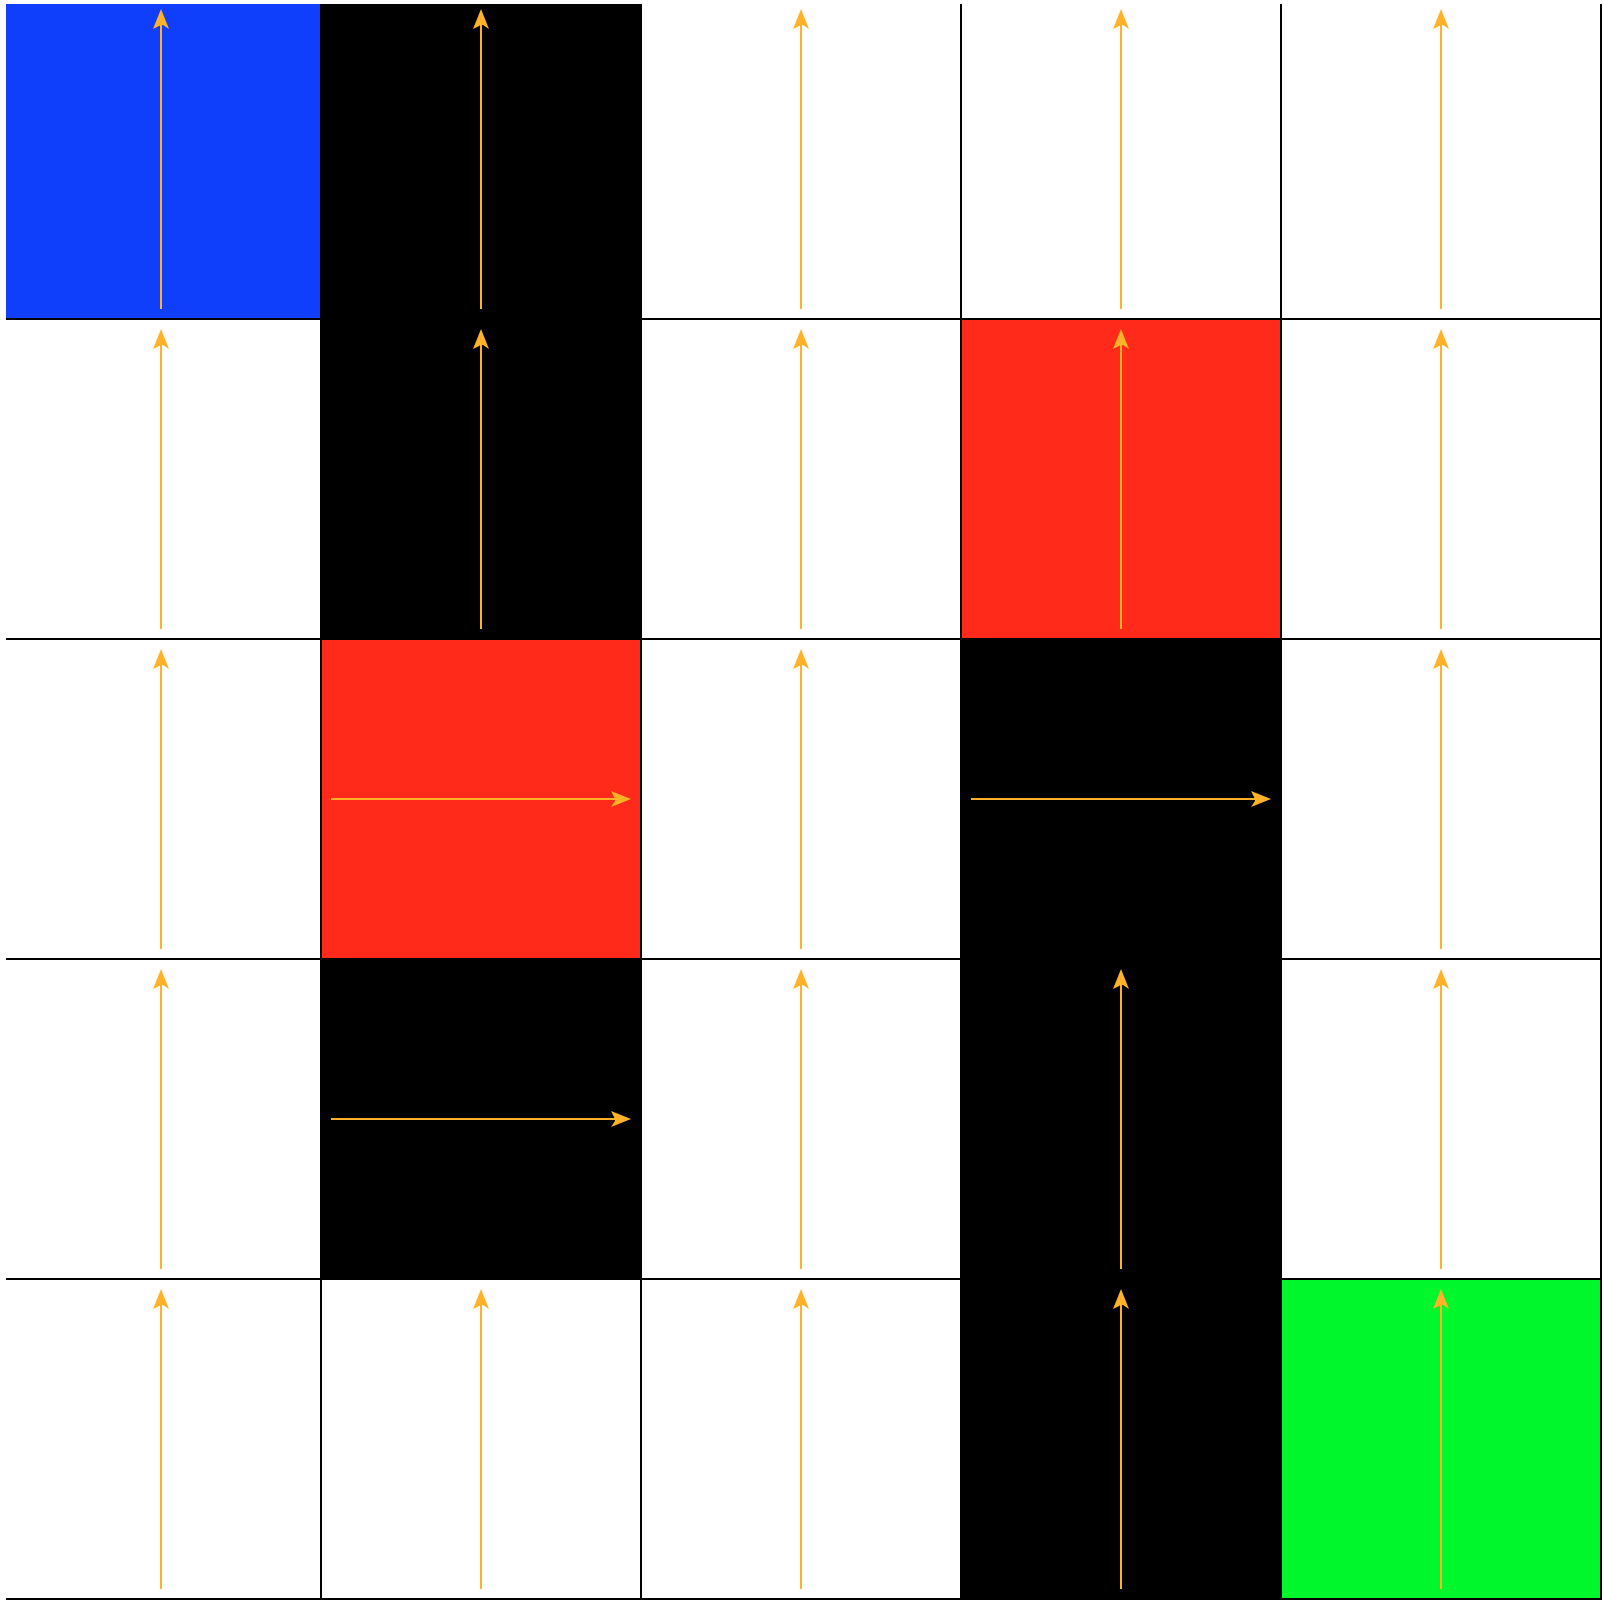
\includegraphics[width=\textwidth]{figures/5x5_viter_r3.png}
                \caption{Reward schema 3\\
                Reward: $\infty$  \\
                Time:  0.0002\\
                Iterations: 2}
                \label{fig:mouse}
        \end{subfigure}
        \caption{Policies Learned by Value Iteration}\label{fig:animals}
\end{figure}

\subsubsection{Policy Iteration}
\begin{figure}[h!]
        \centering
        \begin{subfigure}[b]{0.3\textwidth}
                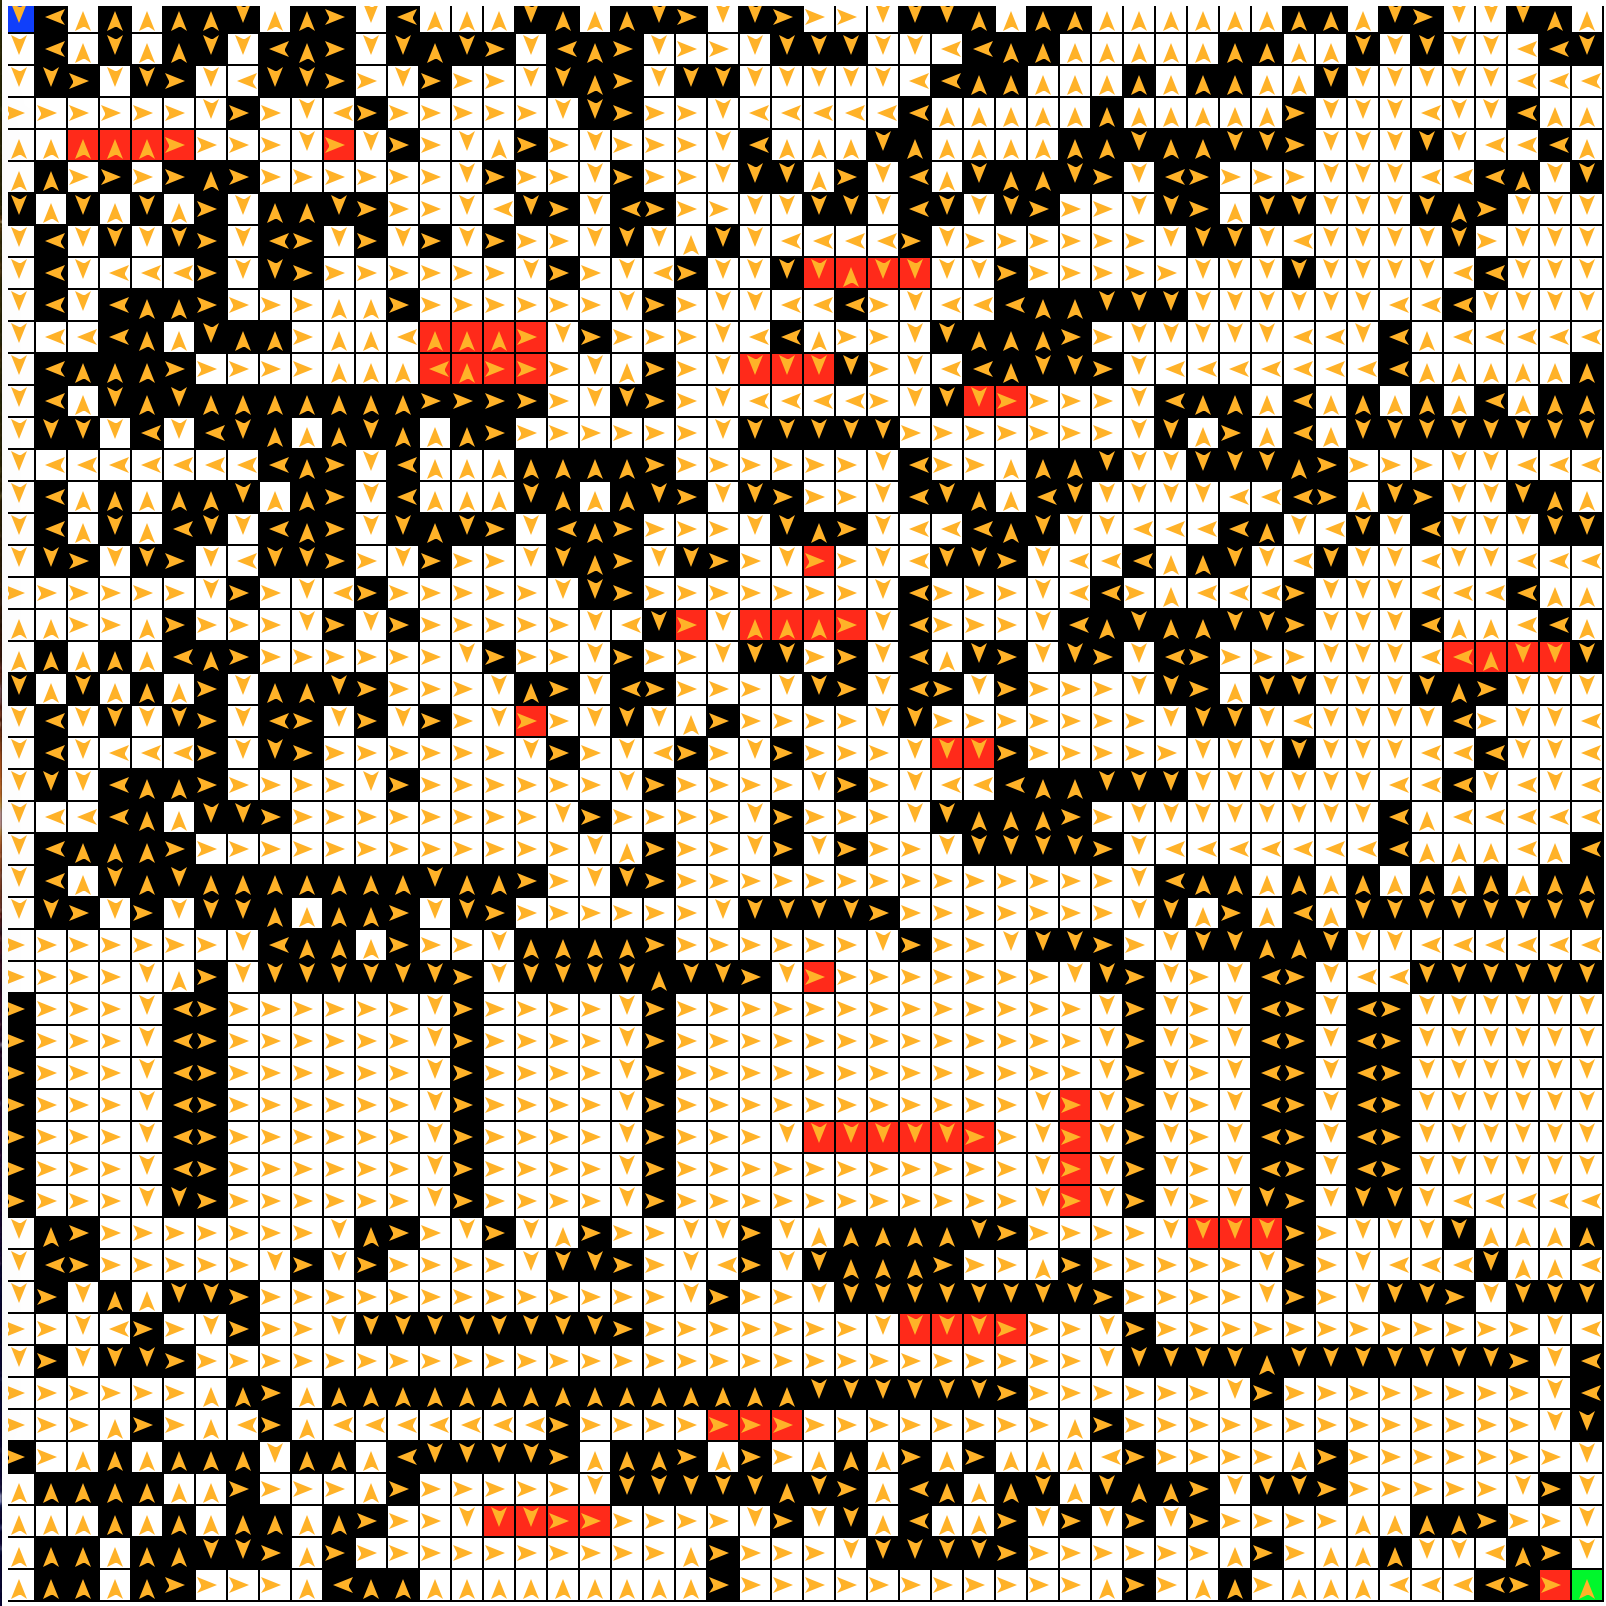
\includegraphics[width=\textwidth]{figures/50x50_piter_r1.png}
                \caption{Reward schema 1\\
                Reward:  995.15 \\
                Time:  39.5257\\
                Iterations: 81 }
                \label{fig:gull}
        \end{subfigure}%
        ~ %add desired spacing between images, e. g. ~, \quad, \qquad, \hfill etc.
          %(or a blank line to force the subfigure onto a new line)
        \begin{subfigure}[b]{0.3\textwidth}
                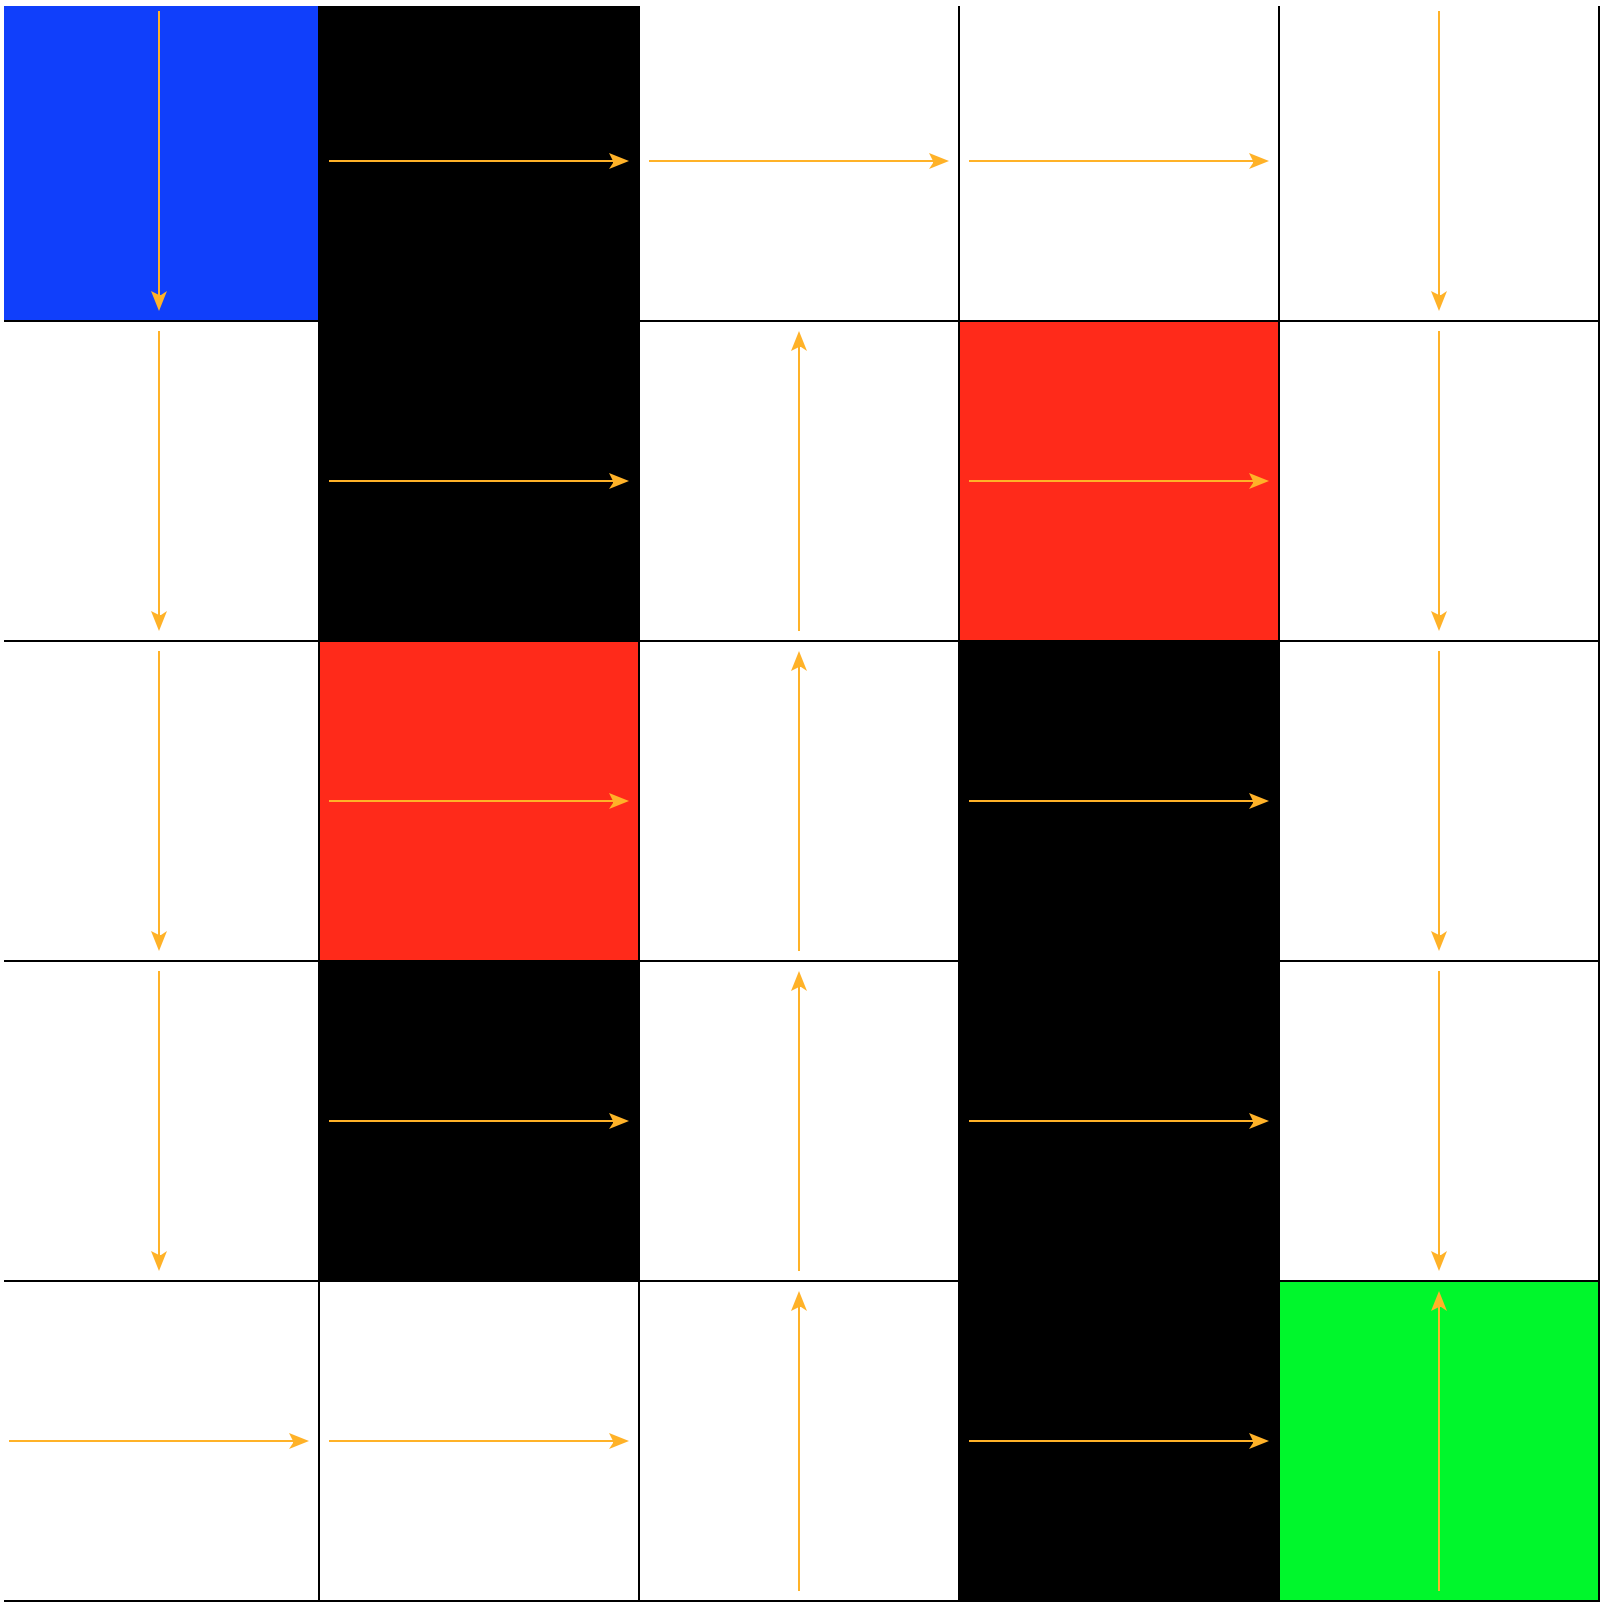
\includegraphics[width=\textwidth]{figures/5x5_piter_r2.png}
                \caption{Reward schema 2\\
                Reward: -5 \\
                Time:  0.0112\\
                Iterations: 11 }
                \label{fig:tiger}
        \end{subfigure}
        ~ %add desired spacing between images, e. g. ~, \quad, \qquad, \hfill etc.
          %(or a blank line to force the subfigure onto a new line)
        \begin{subfigure}[b]{0.3\textwidth}
                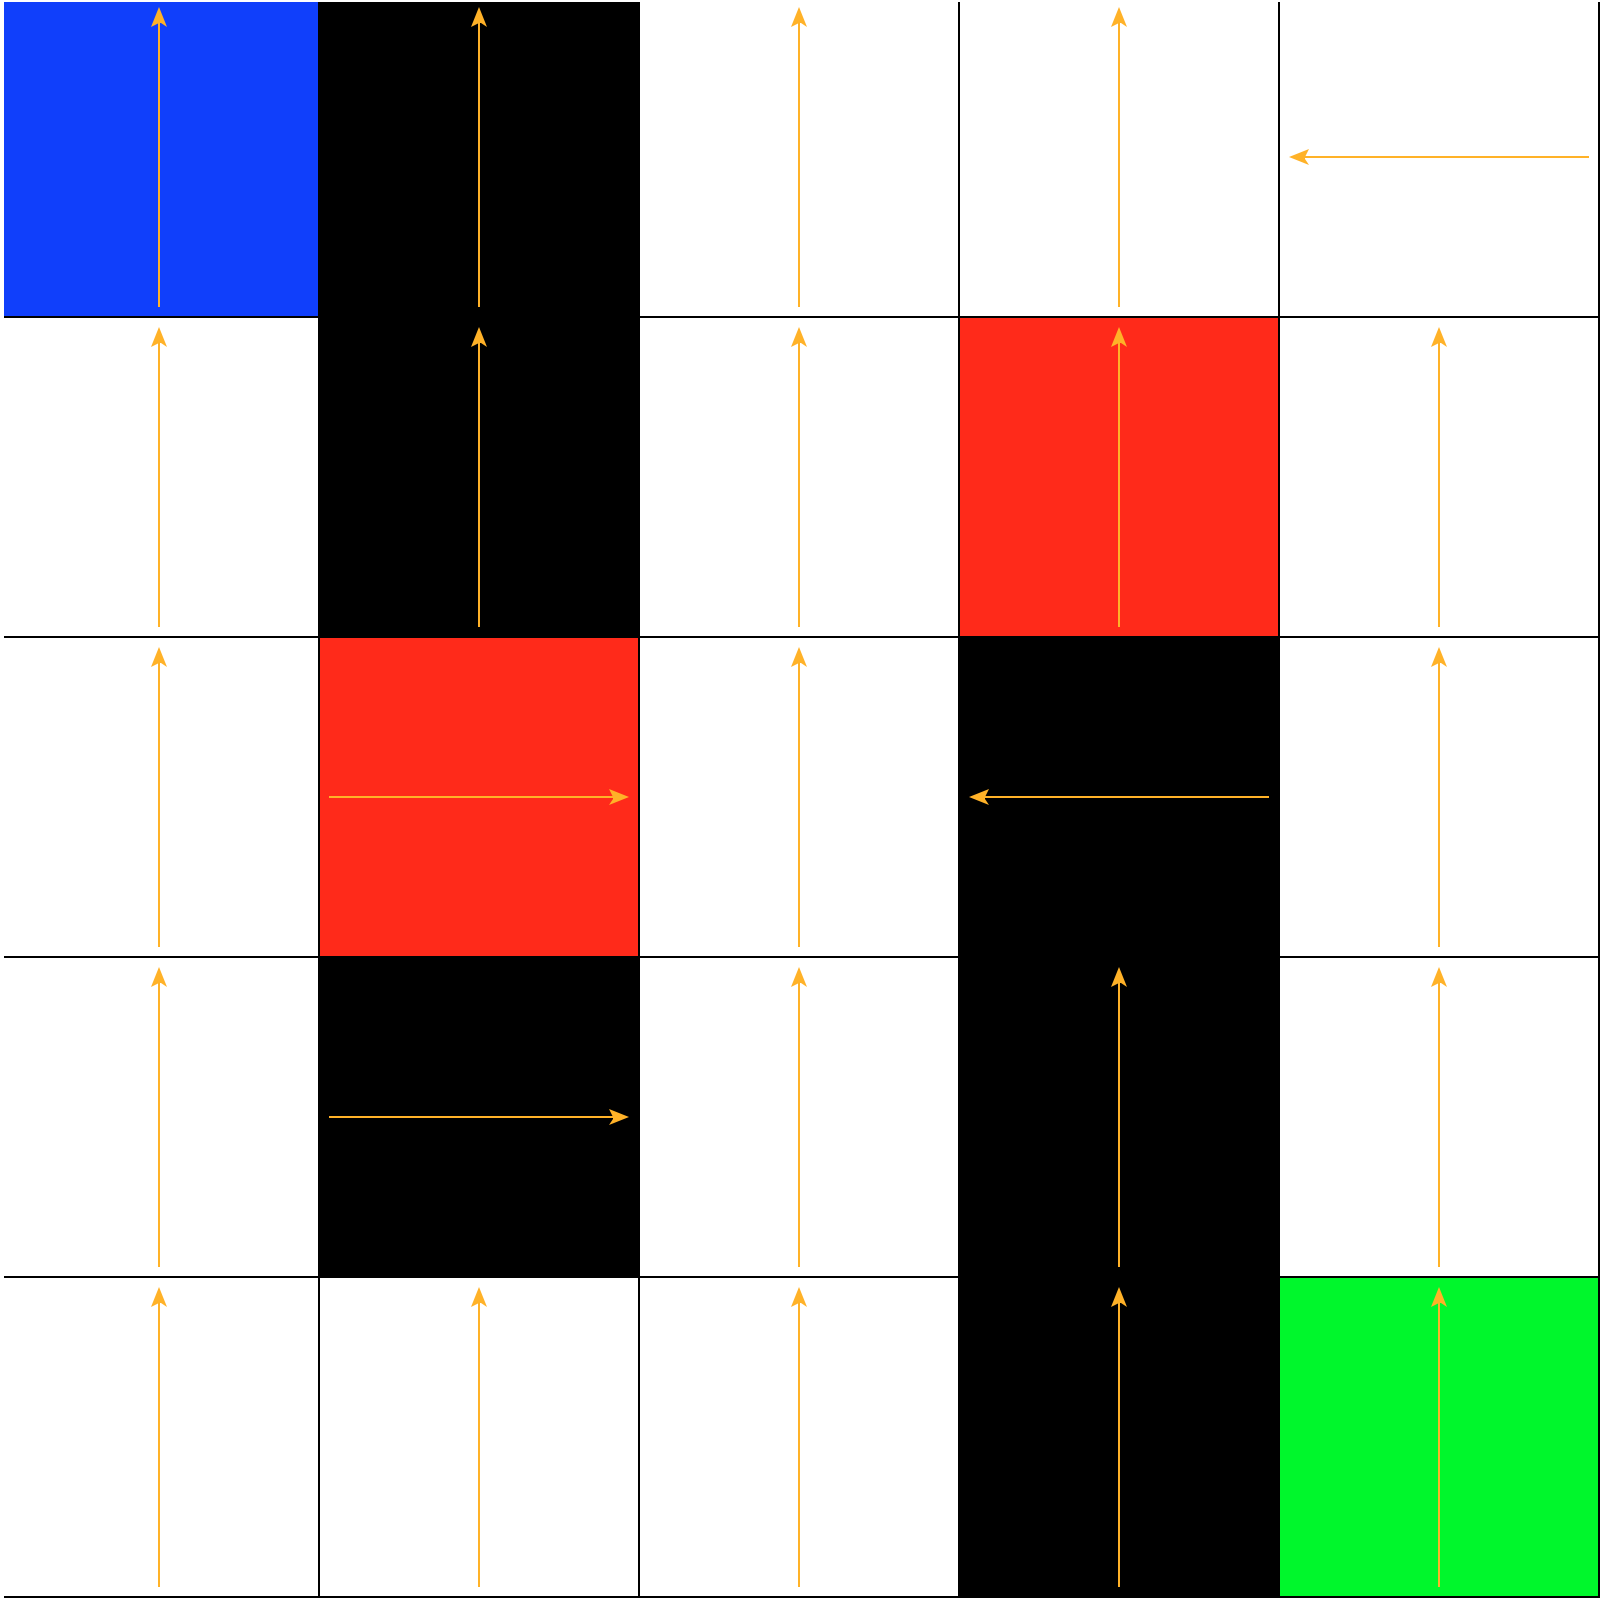
\includegraphics[width=\textwidth]{figures/5x5_piter_r3.png}
                \caption{Reward schema 3\\
                Reward: $\infty$ \\
                Time: 0.5076\\
                Iterations: 1000 (max)}
                \label{fig:mouse}
        \end{subfigure}
        \caption{Policies Learned by Policy Iteration}\label{fig:animals}
\end{figure}

\subsubsection{Q-Learning}
\begin{figure}[h!]
        \centering
        \begin{subfigure}[b]{0.3\textwidth}
                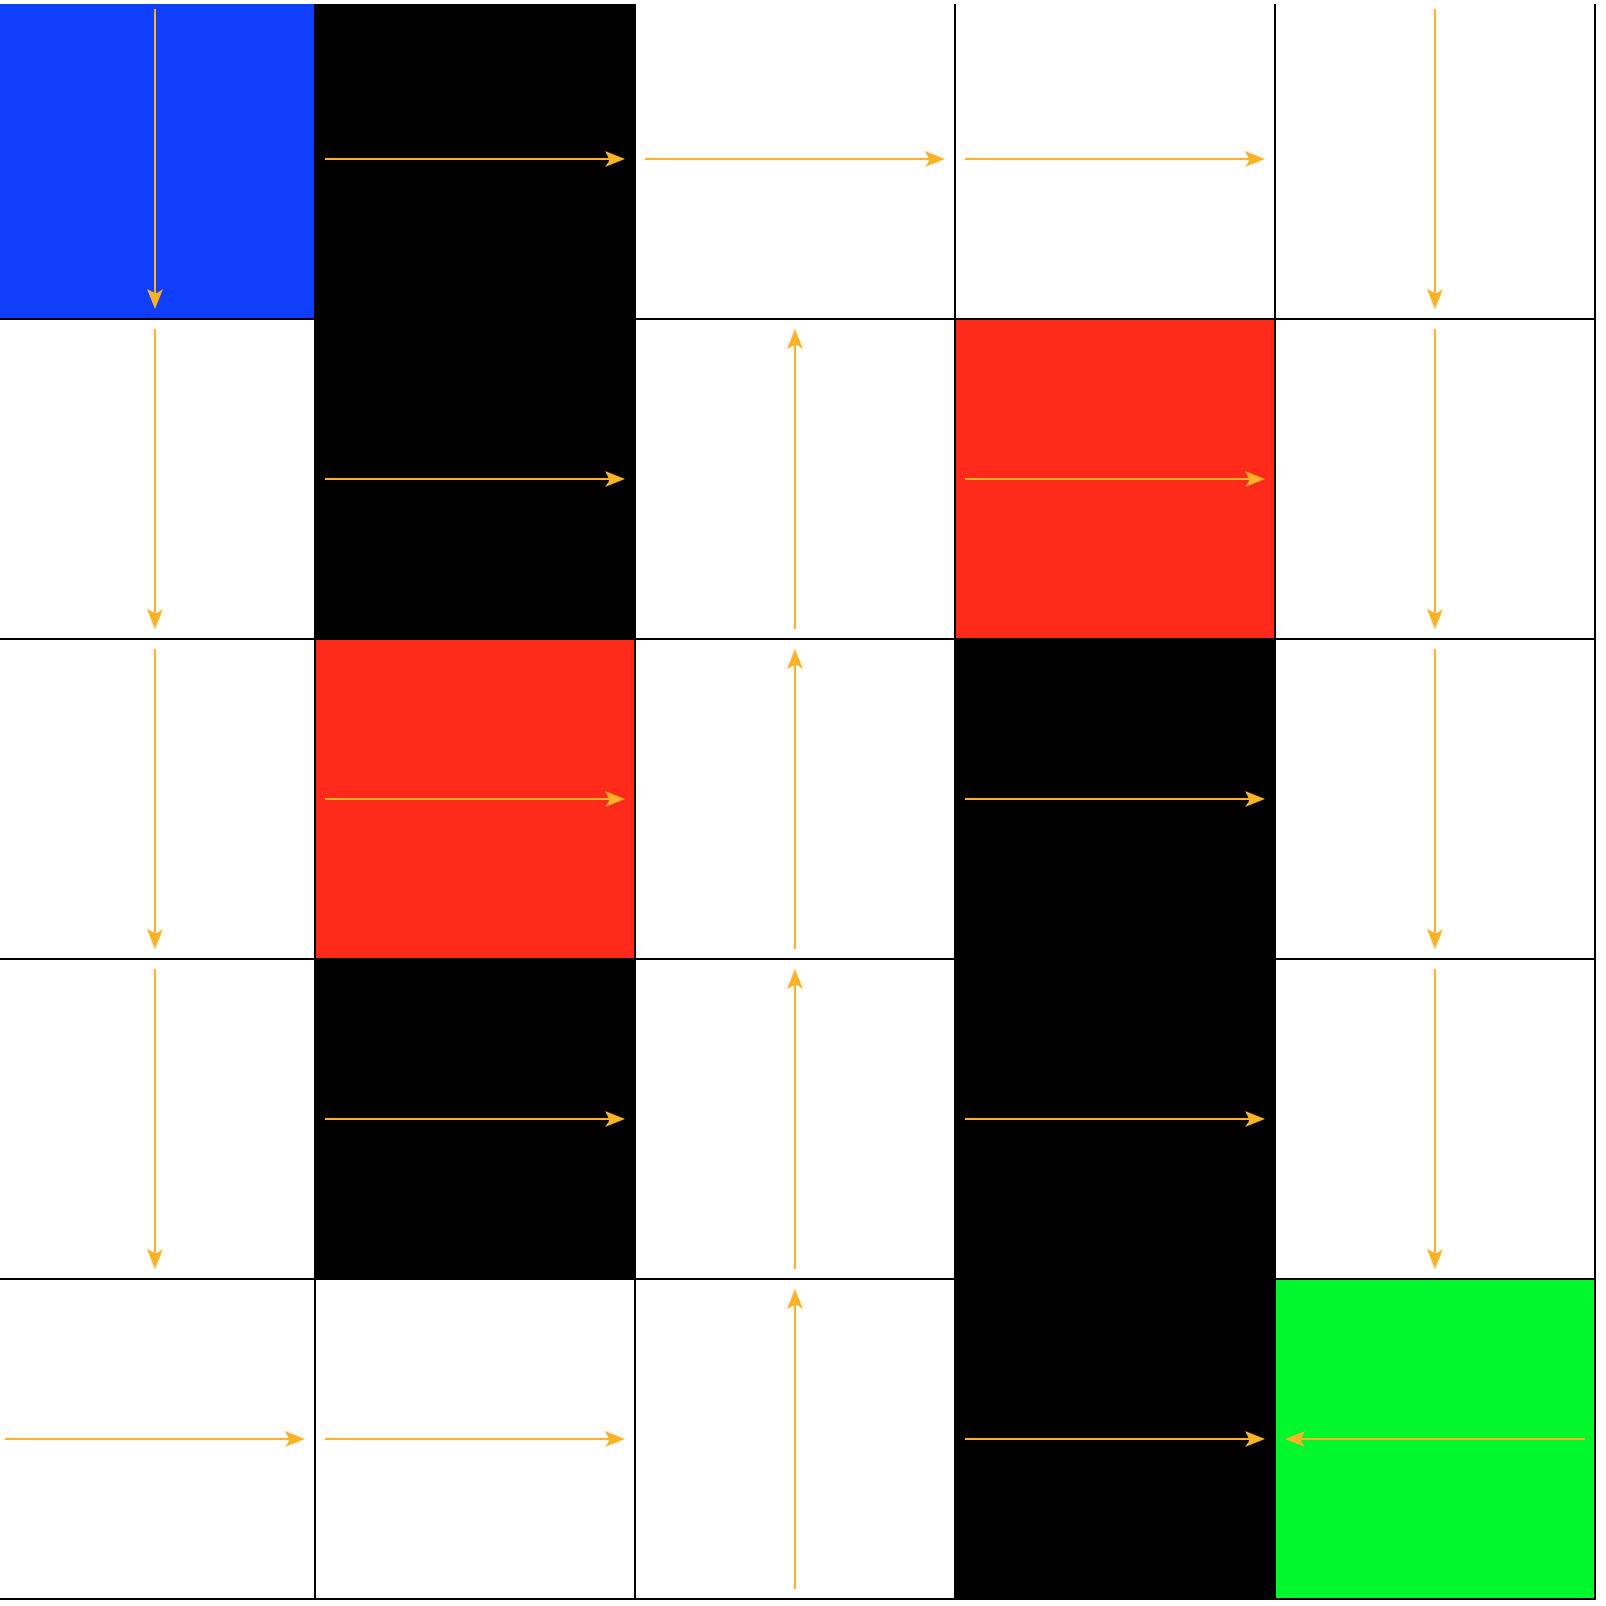
\includegraphics[width=\textwidth]{figures/5x5_qlearn_r1.png}
                \caption{Reward schema 1\\ 
                Reward:  9.25 \\
                Time:  1.353 \\
                Iterations:  25013 }
                \label{fig:gull}
        \end{subfigure}%
        ~ %add desired spacing between images, e. g. ~, \quad, \qquad, \hfill etc.
          %(or a blank line to force the subfigure onto a new line)
        \begin{subfigure}[b]{0.3\textwidth}
                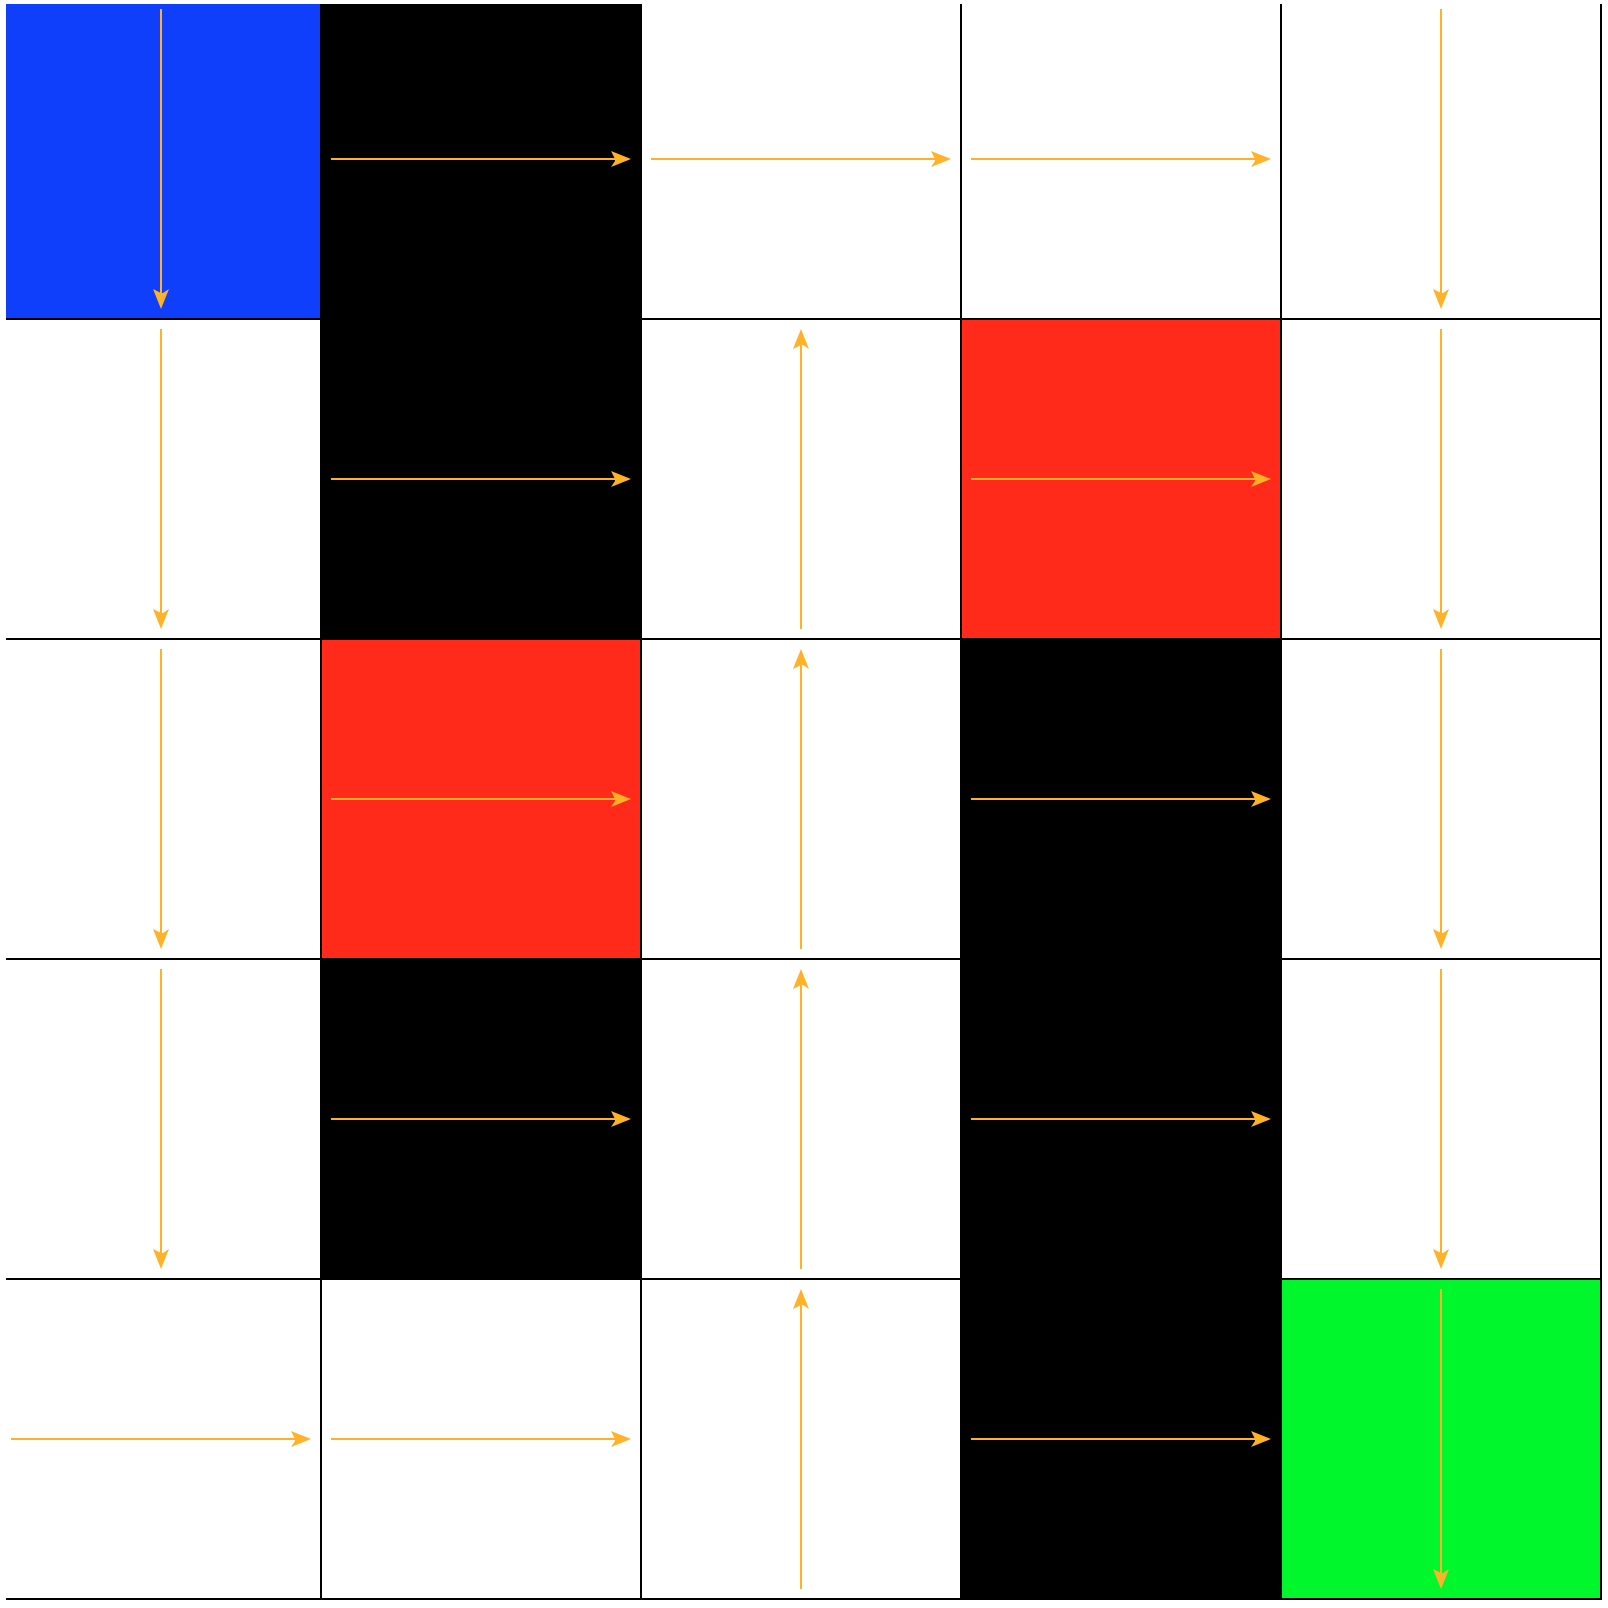
\includegraphics[width=\textwidth]{figures/5x5_qlearn_r2.png}
                \caption{Reward schema 2\\
                Reward: -5\\
                Time:  1.340\\
                Iterations: 25597 }
                \label{fig:tiger}
        \end{subfigure}
        ~ %add desired spacing between images, e. g. ~, \quad, \qquad, \hfill etc.
          %(or a blank line to force the subfigure onto a new line)
        \begin{subfigure}[b]{0.3\textwidth}
                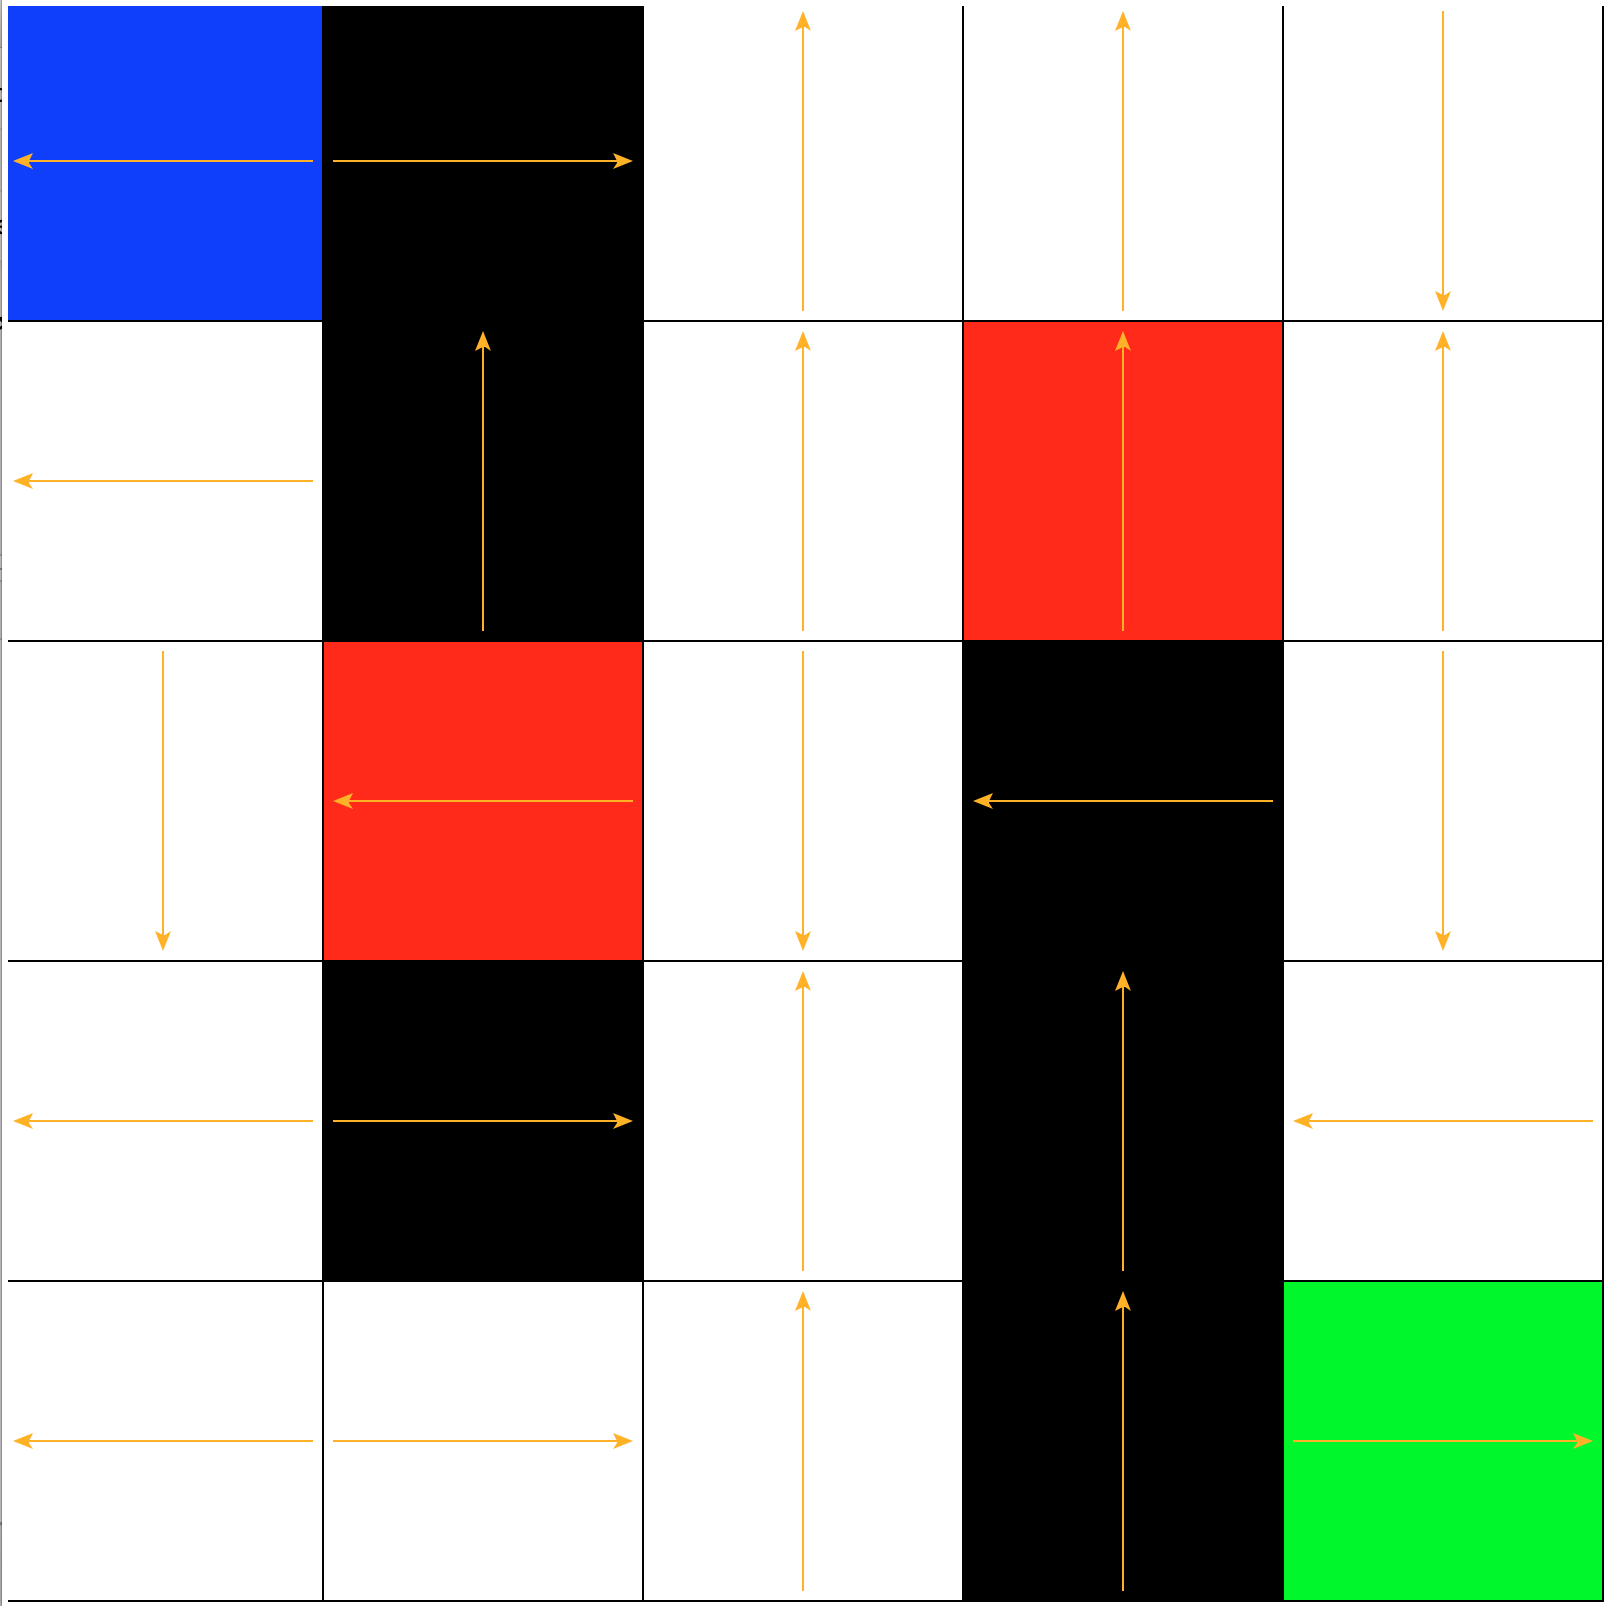
\includegraphics[width=\textwidth]{figures/5x5_qlearn_r3.png}
                \caption{Reward schema 3 \\
                Reward: $\infty$\\
                Time: 1.677 \\
                Iterations: 65465 }
                \label{fig:mouse}
        \end{subfigure}
        \caption{Policies Learned by Q-Learning}\label{fig:animals}
\end{figure}

\end{document}